\documentclass[twocolumn]{article}

% Load basic packages
\usepackage{balance}  % to better equalize the last page
% \usepackage{txfonts}
\usepackage{times}    % comment if you want LaTeX's default font
\usepackage{xcolor}
\usepackage{booktabs}
%\usepackage{ccicons}
\usepackage{float}
\usepackage[hyphens]{url}  
\usepackage{titling}	% allows you to move title up the page
\usepackage[pdftex]{hyperref}
\usepackage{fancyhdr}
% \usepackage[left=2.75cm, right=2.75cm]{geometry}

% \usepackage{caption}
% \usepackage{subcaption}
% \usepackage{subfig}

% graphics
\usepackage{graphicx}
\graphicspath{ {./assets/} }

% equations
\usepackage{amsmath,amssymb}

% font  sizes
\usepackage{sectsty}			% set font sizes			
\sectionfont{\Large}			% (assumes default font size 10pt)
\subsectionfont{\large}
\subsubsectionfont{\large}
\paragraphfont{\normalsize}

% positioning
\setlength{\parindent}{0em}		% remove indent for new paragraph
\setlength{\parskip}{1em}		% space above paragraph
\setlength{\columnsep}{2em}		% distance between columns
\setlength{\droptitle}{-7em}

% llt: Define a global style for URLs, rather that the default one
\makeatletter
\def\url@leostyle{%
  \@ifundefined{selectfont}{\def\UrlFont{\sf}}{\def\UrlFont{\small\bf\ttfamily}}}
\makeatother
\urlstyle{leo}

% pandoc stuff
% \providecommand{\tightlist}{%
%   \setlength{\itemsep}{0pt}\setlength{\parskip}{0pt}}


\makeatletter
\@ifundefined{KOMAClassName}{% if non-KOMA class
  \IfFileExists{parskip.sty}{%
    \usepackage{parskip}
  }{% else
    \setlength{\parindent}{0pt}
    \setlength{\parskip}{6pt plus 2pt minus 1pt}}
}{% if KOMA class
  \KOMAoptions{parskip=half}}
\makeatother
\usepackage{color}
\usepackage{fancyvrb}
\newcommand{\VerbBar}{|}
\newcommand{\VERB}{\Verb[commandchars=\\\{\}]}
\DefineVerbatimEnvironment{Highlighting}{Verbatim}{commandchars=\\\{\}}
% Add ',fontsize=\small' for more characters per line
\newenvironment{Shaded}{}{}
\newcommand{\AlertTok}[1]{\textcolor[rgb]{1.00,0.00,0.00}{\textbf{#1}}}
\newcommand{\AnnotationTok}[1]{\textcolor[rgb]{0.38,0.63,0.69}{\textbf{\textit{#1}}}}
\newcommand{\AttributeTok}[1]{\textcolor[rgb]{0.49,0.56,0.16}{#1}}
\newcommand{\BaseNTok}[1]{\textcolor[rgb]{0.25,0.63,0.44}{#1}}
\newcommand{\BuiltInTok}[1]{\textcolor[rgb]{0.00,0.50,0.00}{#1}}
\newcommand{\CharTok}[1]{\textcolor[rgb]{0.25,0.44,0.63}{#1}}
\newcommand{\CommentTok}[1]{\textcolor[rgb]{0.38,0.63,0.69}{\textit{#1}}}
\newcommand{\CommentVarTok}[1]{\textcolor[rgb]{0.38,0.63,0.69}{\textbf{\textit{#1}}}}
\newcommand{\ConstantTok}[1]{\textcolor[rgb]{0.53,0.00,0.00}{#1}}
\newcommand{\ControlFlowTok}[1]{\textcolor[rgb]{0.00,0.44,0.13}{\textbf{#1}}}
\newcommand{\DataTypeTok}[1]{\textcolor[rgb]{0.56,0.13,0.00}{#1}}
\newcommand{\DecValTok}[1]{\textcolor[rgb]{0.25,0.63,0.44}{#1}}
\newcommand{\DocumentationTok}[1]{\textcolor[rgb]{0.73,0.13,0.13}{\textit{#1}}}
\newcommand{\ErrorTok}[1]{\textcolor[rgb]{1.00,0.00,0.00}{\textbf{#1}}}
\newcommand{\ExtensionTok}[1]{#1}
\newcommand{\FloatTok}[1]{\textcolor[rgb]{0.25,0.63,0.44}{#1}}
\newcommand{\FunctionTok}[1]{\textcolor[rgb]{0.02,0.16,0.49}{#1}}
\newcommand{\ImportTok}[1]{\textcolor[rgb]{0.00,0.50,0.00}{\textbf{#1}}}
\newcommand{\InformationTok}[1]{\textcolor[rgb]{0.38,0.63,0.69}{\textbf{\textit{#1}}}}
\newcommand{\KeywordTok}[1]{\textcolor[rgb]{0.00,0.44,0.13}{\textbf{#1}}}
\newcommand{\NormalTok}[1]{#1}
\newcommand{\OperatorTok}[1]{\textcolor[rgb]{0.40,0.40,0.40}{#1}}
\newcommand{\OtherTok}[1]{\textcolor[rgb]{0.00,0.44,0.13}{#1}}
\newcommand{\PreprocessorTok}[1]{\textcolor[rgb]{0.74,0.48,0.00}{#1}}
\newcommand{\RegionMarkerTok}[1]{#1}
\newcommand{\SpecialCharTok}[1]{\textcolor[rgb]{0.25,0.44,0.63}{#1}}
\newcommand{\SpecialStringTok}[1]{\textcolor[rgb]{0.73,0.40,0.53}{#1}}
\newcommand{\StringTok}[1]{\textcolor[rgb]{0.25,0.44,0.63}{#1}}
\newcommand{\VariableTok}[1]{\textcolor[rgb]{0.10,0.09,0.49}{#1}}
\newcommand{\VerbatimStringTok}[1]{\textcolor[rgb]{0.25,0.44,0.63}{#1}}
\newcommand{\WarningTok}[1]{\textcolor[rgb]{0.38,0.63,0.69}{\textbf{\textit{#1}}}}
\usepackage{longtable,booktabs,array}
\usepackage{calc} % for calculating minipage widths
% Correct order of tables after \paragraph or \subparagraph
\usepackage{etoolbox}
\makeatletter
\patchcmd\longtable{\par}{\if@noskipsec\mbox{}\fi\par}{}{}
\makeatother
% Allow footnotes in longtable head/foot
\IfFileExists{footnotehyper.sty}{\usepackage{footnotehyper}}{\usepackage{footnote}}
\makesavenoteenv{longtable}
% definitions for citeproc citations
\NewDocumentCommand\citeproctext{}{}
\NewDocumentCommand\citeproc{mm}{%
  \begingroup\def\citeproctext{#2}\cite{#1}\endgroup}
\makeatletter
 % allow citations to break across lines
 \let\@cite@ofmt\@firstofone
 % avoid brackets around text for \cite:
 \def\@biblabel#1{}
 \def\@cite#1#2{{#1\if@tempswa , #2\fi}}
\makeatother
\newlength{\cslhangindent}
\setlength{\cslhangindent}{1.5em}
\newlength{\csllabelwidth}
\setlength{\csllabelwidth}{3em}
\newenvironment{CSLReferences}[2] % #1 hanging-indent, #2 entry-spacing
 {\begin{list}{}{%
  \setlength{\itemindent}{0pt}
  \setlength{\leftmargin}{0pt}
  \setlength{\parsep}{0pt}
  % turn on hanging indent if param 1 is 1
  \ifodd #1
   \setlength{\leftmargin}{\cslhangindent}
   \setlength{\itemindent}{-1\cslhangindent}
  \fi
  % set entry spacing
  \setlength{\itemsep}{#2\baselineskip}}}
 {\end{list}}
\usepackage{calc}
\newcommand{\CSLBlock}[1]{\hfill\break\parbox[t]{\linewidth}{\strut\ignorespaces#1\strut}}
\newcommand{\CSLLeftMargin}[1]{\parbox[t]{\csllabelwidth}{\strut#1\strut}}
\newcommand{\CSLRightInline}[1]{\parbox[t]{\linewidth - \csllabelwidth}{\strut#1\strut}}
\newcommand{\CSLIndent}[1]{\hspace{\cslhangindent}#1}
\setlength{\emergencystretch}{3em} % prevent overfull lines
\providecommand{\tightlist}{%
  \setlength{\itemsep}{0pt}\setlength{\parskip}{0pt}}
\usepackage{graphicx}
\graphicspath{ {./assets/} }

\usepackage{fvextra}
\DefineVerbatimEnvironment{Highlighting}{Verbatim}{breaklines,commandchars=\\\{\}}

\usepackage{longtable}
\usepackage{multirow}
\makeatletter
\@ifpackageloaded{subfig}{}{\usepackage{subfig}}
\@ifpackageloaded{caption}{}{\usepackage{caption}}
\captionsetup[subfloat]{margin=0.5em}
\AtBeginDocument{%
\renewcommand*\figurename{Figure}
\renewcommand*\tablename{Table}
}
\AtBeginDocument{%
\renewcommand*\listfigurename{List of Figures}
\renewcommand*\listtablename{List of Tables}
}
\newcounter{pandoccrossref@subfigures@footnote@counter}
\newenvironment{pandoccrossrefsubfigures}{%
\setcounter{pandoccrossref@subfigures@footnote@counter}{0}
\begin{figure}\centering%
\gdef\global@pandoccrossref@subfigures@footnotes{}%
\DeclareRobustCommand{\footnote}[1]{\footnotemark%
\stepcounter{pandoccrossref@subfigures@footnote@counter}%
\ifx\global@pandoccrossref@subfigures@footnotes\empty%
\gdef\global@pandoccrossref@subfigures@footnotes{{##1}}%
\else%
\g@addto@macro\global@pandoccrossref@subfigures@footnotes{, {##1}}%
\fi}}%
{\end{figure}%
\addtocounter{footnote}{-\value{pandoccrossref@subfigures@footnote@counter}}
\@for\f:=\global@pandoccrossref@subfigures@footnotes\do{\stepcounter{footnote}\footnotetext{\f}}%
\gdef\global@pandoccrossref@subfigures@footnotes{}}
\@ifpackageloaded{float}{}{\usepackage{float}}
\floatstyle{ruled}
\@ifundefined{c@chapter}{\newfloat{codelisting}{h}{lop}}{\newfloat{codelisting}{h}{lop}[chapter]}
\floatname{codelisting}{Listing}
\newcommand*\listoflistings{\listof{codelisting}{List of Listings}}
\makeatother
\usepackage{bookmark}
\IfFileExists{xurl.sty}{\usepackage{xurl}}{} % add URL line breaks if available
\urlstyle{same}
\hypersetup{
  pdftitle={The Good, the Bad and the Noisy: Acoustic Features in Cross-Domain Argument Mining},
  pdfauthor={Oscar Morris},
  hidelinks,
  pdfcreator={LaTeX via pandoc}}

%%%%%%%%%%%%%%%%%%%%%%%%%%%%%%%
% END OF STYLES 
%%%%%%%%%%%%%%%%%%%%%%%%%%%%%%%

% TITLE
\title{The Good, the Bad and the Noisy: Acoustic Features in
Cross-Domain Argument Mining}
\author{Oscar
Morris\\ID: 2497790\\AC40001 Honours Project\\BSc (Hons) Computing Science\\University of Dundee\\Supervisor: Dr.~R.
Ruiz-Dolz}
\date{April 2025\vspace{5ex}}

% headers
\pagestyle{fancy}
\fancyhf{}
\renewcommand{\headrulewidth}{0pt}
\fancyhead[LO]{{\footnotesize The Good, the Bad and the Noisy: Acoustic
features in Cross-Domain Argument Mining}}
\fancyhead[RE]{{\footnotesize Oscar Morris}}
\fancyfoot[C]{\thepage}



%%%%%%%%%%%%%%%%%%%%%%%%%%%
% MAIN DOCUMENT STARTS HERE
%%%%%%%%%%%%%%%%%%%%%%%%%%%

% BEGIN DOCUMENT
\begin{document}

% add title
\maketitle
\raggedbottom


%%%%%%%%%%%
%%%%%%%%%%%
\begin{abstract}
Recent advances in argument relation identification have begun to look
beyond the domain in which they were trained such that these systems can
robustly deal with the wide variety of domains they would see in a
practical application. In many domains, the data stem from a dialogue
(e.g.~political debates), the additional paralinguistic features present
in the audio data have, until recently, gone unexplored. Work exploring
the addition of acoustic data has previously been hampered by a lack of
available corpora. In this project, the largest multimodal argument
relation identification dataset currently available is presented, along with a
cross-domain dataset. These datasets are then used to evaluate nine
different multimodal techniques in both an in-domain and a cross-domain
environment. It was found that while the addition of acoustic features
does not provide a significant improvement over text only solutions, the
process used to combine the data from each sequence in the pair is
vitally important to the performance of the model.
\end{abstract}

%%%%%%%%%%%
%%%%%%%%%%%

\section{Introduction}\label{introduction}

Argument relation identification (ARI) is a subtask of argument mining
(AM) involved with the detection and classification of the argumentative
components contained within text and discussion {[}1{]}. AM generally
can cover many different tasks, including argumentative sequence
detection, argument component classification and ARI in a specific
domain. All of these tasks (often when combined) have many different
applications such as fake news {[}2{]} and \mbox{fallacy detection {[}3{]}}
with uses across many fields including political science, military and
corporate intelligence, and education. In all of these fields, it is
important to be able to extract arguments and their relations accurately
and with ease.

In many contexts (e.g.~political debates or court proceedings) both the
audio and textual data exist, where typically the text has been
transcribed from the audio. Previously, most argument mining systems
have focused completely on the textual data, often gained from a
transcript of these discussions or debates. More recent research,
however, has shown that the paralinguistic features available from other
modalities of data (either images or audio) are able to improve the
performance over text only solutions {[}4{]}.

Multimodal models have shown the greatest level of improvement in
argumentative sentence detection and argument segmentation {[}5{]}.
However, they have only had varying degrees of success in ARI with
Mancini \emph{et al.} {[}6{]} finding the addition of acoustic features
significantly increased performance while Mestre \emph{et al.} {[}7{]}
find no significant difference. Recent advances in multimodal models and
their pre-training have now allowed the effective addition of \mbox{acoustic
features {[}8, 9{]}}, along with advances in other areas of natural
language processing, more specifically, the advent of the transformer
{[}10{]} and the recent boom of large language models (LLMs), including
their use in text-based argument mining {[}11{]}. Due to their size,
LLMs perform very well across a variety of domains and fields, but at
great computational cost. Therefore, it is pertinent to understand how
smaller models perform across a number of domains.

Traditionally, AM systems have been evaluated on the same domain that
they were trained on {[}12, 13{]}. But given the recent uses of
relatively task agnostic pre-training approaches and models such as BERT
{[}14{]} and then the advent of LLMs has further increased the need for
domain agnostic models. These advancements have also been applied to
argument mining by evaluating models on datasets and domains with which
they were not trained {[}15, 16{]}. This approach has not yet been
evaluated on multimodal models generally nor text-audio models
specifically, in any sub-task of argument mining, it is very possible
that the addition of acoustic features will be helpful for the model to
learn more intrinsic, less domain-specific features and therefore
increase its ability to generalise beyond the domain in which it was
trained. A likely reason that this has not been studied further is the
relative lack of resources and available datasets designed for
text-audio ARI. The only datasets currently available for the task are
the M-Arg political debate dataset {[}7{]} with 7 hours of audio data,
and the VivesDebate-Speech dataset {[}5{]} with 12 hours of audio data.
Although they are the largest text-audio datasets of their type which
are currently available, when comparing to the large text only datasets
they are still relatively small. For example, M-Arg and
Vivesdebate-Speech contain 6,527 and 7,810 nodes with one of the largest
debate datasets, \mbox{QT30 {[}17{]}} containing almost 20,000. This difference
in size means that there is still significant room for multimodal ARI
datasets to grow and hints at a limitation surrounding the current
approaches and models.

It is for this reason that the goals of this project are twofold:

\begin{enumerate}
\def\labelenumi{(\roman{enumi})}
\tightlist
\item
  Extend two existing debate corpora with their audio data, allowing
  their use for all multimodal or audio only AM applications. The first
  of these is the large QT30 corpus {[}17{]} and the second is a
  smaller, but cross-domain corpus created from Moral Maze episodes
  {[}18{]}.
\item
  The implementation and evaluation of different multimodal techniques
  and models in a cross-domain setting on the task of argument relation
  identification.
\end{enumerate}

\section{Background}\label{background}

\subsection{Argumentation Theory}\label{argumentation-theory}

Argument and debate has been studied since the time of the ancient Greek
philosophers and rhetoricians where argument theorists have sought to
formalise discourse and discover some standard of proof for determining
the `correctness' of an argument. Over time, theories of arguments and
discussions have evolved, notably when Hamblin {[}19{]} refashioned an
argumentative discourse as a game, where one party makes moves offering
premises that may be acceptable to the another party in the discourse
who doubts the conclusion of the argument. When viewing a discourse as a
game, it becomes possible to model discourse in such a way that it can
be viewed through the lens of formal logic, and therefore
computationally too.

In order to describe various dialogue, argument and illocutionary
structures different models (annotation schemes) can be used, some
annotation schemes focus on types of the text itself (such as speech act
theory {[}20{]}) or on the types of relations between components (such
as Rhetorical Structure Theory {[}21{]}). Inference Anchoring Theory
(IAT) {[}22{]} is an annotation scheme constructed to benefit from
insights across both types, whilst focusing specifically on
argumentative discourse. This makes IAT a very useful tool to analyse
arguments and their relations.

In IAT, the discourse is first segmented into Argumentative Discourse
Units (ADUs). An ADU is any span of the discourse which has both
propositional content and discrete argumentative function {[}23{]}. An
IAT argument graph is typically composed of two main parts: the
left-hand side and the right-hand side. The right-hand side is concerned
with locutions and transitions between them. A locution is simply the
text of the ADU as uttered, without reconstructing ellipses or resolving
pronouns. Locutions also include the speaker and may even include a
timestamp. Transitions connect locutions capturing a functional
relationship between predecessor and successor locutions (i.e.~a
response or reply). The left-hand side of an argument graph is more
concerned with the content of the ADU, rather than directly reflecting
what was uttered. This consists of the propositions made, and the
relations between those propositions. To create a proposition from an
ADU, the content is reconstructed to be a coherent, lone-standing
sentence. This means that any missing or implicit material has to be
reconstructed, including anaphoric references (e.g.~pronouns).
Performing this reconstruction allows both a human annotator and a
computational system to view some of the context surrounding the
locution and therefore make a better judgement as to a proposition's
relation to others.

IAT defines three different types of propositional relation:
\emph{inference}, \emph{conflict} and \emph{rephrase}. An inference
relation (also termed RA) holds between two propositions when one (the
premise) is used to provide a reason to accept the other (the
conclusion). This may include annotation of the kind of support
e.g.~Modus Ponens or Argument from Expert Opinion. These subtypes of
relation are often called \mbox{\emph{argument schemes} {[}24, 25{]}.}
There are also several different inference structures (images from
{[}1{]}):

\begin{itemize}
\tightlist
\item
  \textbf{Serial arguments} occur when one proposition supports another,
  which in turn supports a third.
\end{itemize}

\begin{figure}[H]
    \centering
    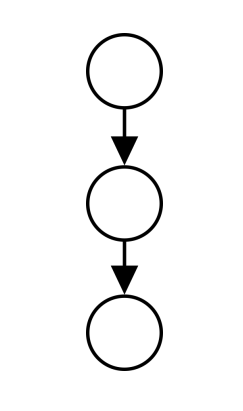
\includegraphics[height=2cm]{serial}
\end{figure}

\begin{itemize}
\tightlist
\item
  \textbf{Convergent arguments} occur when multiple premises act
  independently to support the same conclusion.
\end{itemize}

\begin{figure}[H]
    \centering
    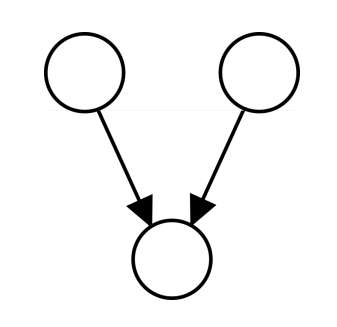
\includegraphics[height=2cm]{convergent}
\end{figure}

\begin{itemize}
\tightlist
\item
  \textbf{Linked arguments} occur when multiple premises work together
  to support a conclusion.
\end{itemize}

\begin{figure}[H]
    \centering
    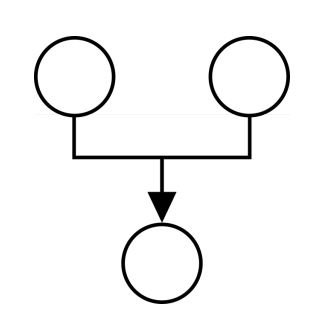
\includegraphics[height=2cm]{linked}
\end{figure}

\begin{itemize}
\tightlist
\item
  \textbf{Divergent arguments} occur when a single premise is used to
  support multiple conclusions.
\end{itemize}

\begin{figure}[H]
    \centering
    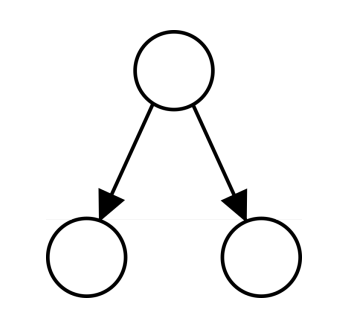
\includegraphics[height=2cm]{divergent}
\end{figure}

A conflict relation (also termed CA) holds between two propositions when
one is used to provide an incompatible alternative to another and can
also be of a given kind (e.g.~Conflict from Bias, Conflict from
Propositional Negation). The following conflict structures are
identified by IAT:

\begin{itemize}
\tightlist
\item
  \textbf{Rebutting conflict} occurs if one proposition is directly
  targeting another by indicating that the latter is not acceptable.
\item
  \textbf{Undermining conflict} occurs if a conflict is targeting the
  premise of an argument, then it is undermining its conclusion.
\item
  \textbf{Undercutting conflict} occurs if the conflict is targeting the
  inference relation between two propositions.
\end{itemize}

A rephrase relation (also termed MA) holds when one proposition
rephrases, restates or reformulates another but with different
propositional content (i.e.~one proposition cannot simply repeat the
other). There are many different kinds of rephrase, such as
Specialisation, Generalisation, Instantiation etc. Generally, question
answering will often involve a rephrase because the propositional
content of the question is typically instantiated, resolved or refined
by its answer. In contrast to inference, conflict and rephrase
structures only have a single incoming an one outgoing edge.

The left and right-hand sides are connected by \emph{illocutionary
connections}. These illocutionary connections are based on illocutionary
force as introduced by speech act theory {[}20{]}. The speech act
\(F(p)\) is the act which relates the locution and and the propositional
content \(p\) through the illocutionary force \(F\) e.g.~asserting
\(p\), requesting \(p\), promising \(p\) etc. There are many diferent
types of illocutionary connection, including: assertions, questions,
challenges, concessions and (dis-)affirmations {[}26{]}. By modelling
these relations it is possible to gain a better understanding of how
something is said and its purpose within the discourse. In doing this,
we create a graph (known as an \emph{argument map}) which can then be
stored computationally.

Several ways to store argumentative data have been created, for example
Argument Markup Language (AML) {[}27{]}, an XML-based language used to
describe arguments in the Araucaria software. More recently, the
Argument Interchange Format (AIF) {[}28{]} has been created to
standardise the storage of IAT graphs.

AIF treats all relevant parts of the argument as nodes within a graph.
These nodes can be put into two categories: \emph{information nodes}
(I-nodes) and \emph{scheme nodes} (S-nodes). I-nodes represent the
claims made in the discourse whereas S-nodes indicate the application of
an argument scheme. Initially I-nodes only included the propositions
made {[}28{]}, but when Reed \emph{et al.} {[}29{]} extended AIF to
cater to dialogues, they added L-nodes as a subclass of I-nodes to
represent locutions. For the purposes of this research, I-nodes and
L-nodes are considered separate classes where I-nodes contain
propositions and L-nodes contain locutions.

Since AIF data can be easily shared, it became the basis for a Worldwide
Argument Web (WWAW) {[}30{]}. Since then, many corpora have been
annotated using IAT and published on the AIFdb\footnote{\url{https://www.aifdb.org/}}
{[}31{]} providing a very useful resource for argumentation research of
many kinds.

\subsection{Natural Language Processing}\label{sec:background-ml}

In recent years there have been several major advances in the field of
natural language processing (NLP), most notably the introduction of the
transformer architecture {[}10{]}. The transformer architecture, based
on self-attention, allows the model to determine much longer range
dependencies than previous approaches. In doing so, the model is able to
learn from the context surrounding a word, even gaining insight from
context `far away' in the text.

Even before Vaswani \emph{et al.} introduced the transformer
architecture supervised and semi-supervised pre-training approaches were
already being explored, and proven to be a very useful tool for
improving the performance of language models {[}32, 33{]}. When
the transformer was introduced these pre-training techniques were
adapted for use in transformers creating models which are able to be
fine-tuned with relatively minimal effort and compute to allow high
performance on a wide variety of \mbox{tasks {[}14, 34{]}.} The
pre-training approaches introduced by BERT and RoBERTa use a combination
of masked language modelling (where the model is trained to predict the
token hidden under a \texttt{{[}mask{]}} token) and next sentence
prediction. The models are then trained using this approach on large
datasets (the dataset used to pre-train RoBERTa totals over 160GB of
uncompressed text).

Transformer models have recently become much more well-known due to the
introduction of Large Language Models (LLMs) such as GPT-4 {[}35{]} and
LLaMA {[}36{]}. LLMs have proven very useful across NLP due to their
ability to achieve high performance on many tasks without the need for
fine-tuning, this can, however, include few-shot techniques to allow
them to `learn' at inference time {[}37, 38{]}.

A similar progression can be seen in the development of audio models.
Pre-training was notably introduced into speech recognition with wav2vec
{[}8{]}, where the model is trained to predict future samples from a
given signal. The wav2vec model has two main stages, first raw audio
samples are fed into a convolutional network which performs a similar
role to the tokenisation seen in text-based language models by using a
sliding window approach to downsample the audio data. These encodings
are then fed into a second convolutional network to create a final
encoding for the sequence.

Transformer models were introduced into the architecture of audio models
with wav2vec2 {[}39{]} and HuBERT {[}40{]}, where the second
convolutional model is replaced with a transformer in order to better
learn dependencies across the entire sequence. These models are then
pre-trained on significant amounts of audio data (960 hours in the case
of wav2vec2) in order to then be fine-tuned on a downstream task. It is
also possible to combine text and audio in order to gain insights from
both modalities.

Combining modalities (such as text and audio) has also proven to be a
useful tool across several tasks, including medical imaging {[}41, 42{]}
and natural language processing {[}43, 44{]}, including
argument mining {[}6, 7{]}. Generally fusion techniques can be
split into two categories: early and late. Early fusion techniques
combine representations of each modality before being used as input to
an encoder, with the primary benefit that only a single encoder is used.
Late fusion techniques use a separate encoder for each modality, and the
encodings are then fused to provide a crossmodal representation of the
input.

In early fusion the input representations are transformed into a common
information space, often using vectorisation techniques dependent on the
modality. Late fusion techiques allow for the encodings of each modality
to be combined in several different ways, often either simple operations
(such as concatenation or an element-wise product) but a cross-modal
attention module can also be used to combine the modalities {[}45, 46{]}.
The fusion techniques used in this project are explained in
detail in Section \ref{sec:models}.

\subsection{Argument Mining}\label{argument-mining}

Various NLP techniques have been beneficial to AM, from statistical
methods to the more recent neural networks, in particular the
transformer architecture {[}15{]}. Before discussing the automation of
AM, it is useful to understand how argument analysis is conducted
manually. Manual argument analysis considers the following steps:

\begin{itemize}
\tightlist
\item
  \textbf{Text Segmentation} involves the splitting of the original
  text/discourse into the pieces that will form the resulting argument
  structure. These pieces are often termed Elementary Discourse Units
  (EDUs).
\item
  \textbf{Argument / Non-Argument Classification} is the task of
  determining which of the segments found in the text segmentation step
  are relevant to the argument. For most manual analysis, this step is
  performed in conjunction with text segmentation i.e.~the analyst
  doesn't segment parts of the text which are not relevant to the
  argument.
\item
  \textbf{Simple Structure} is the identification of relations between
  the arguments (e.g.~inference, conflict and rephrase) and their
  structures (e.g.~convergent, serial etc.).
\item
  \textbf{Refined Structure} refers to the identification of
  argumentation schemes (e.g.~Argument from Expert Opinion, Conflict
  From Bias etc.).
\end{itemize}

When the argument analysis process is automated, the stages are very
similar to those in the manual process. Lawrence and Reed {[}1{]} define
the steps as follows, increasing in computational complexity:

\begin{itemize}
\tightlist
\item
  \textbf{Identifying Argument Components} combines the stages of text
  segmentation and argument / non-argument classification in the manual
  process.
\item
  \textbf{Identifying Clausal Properties} involves the identification of
  both intrinsic clausal properties (e.g.~is X evidence?, is X reported
  speech?) of the ADU and the contextual properties (e.g.~is X a
  premise?, is X a conclusion?).
\item
  \textbf{Identifying Relational Properties} relates to the
  identification of \emph{general relations} between ADUs (e.g.~is X a
  premise for Y?, is X in conflict with Y?) and the identification of
  argument schemes.
\end{itemize}

Generally these stages of AM are not directly used in the literature,
but instead a set of AM sub-tasks which map onto each of these stages,
these tasks are defined by Mancini et \emph{al.} {[}6{]} as follows:

\begin{itemize}
\tightlist
\item
  \textbf{Argumentative Sentence Detection (ASD)} is the task of
  classifying a sequence as containing an argument, or not. ASD can be
  extended to include the task of claim detection, where a sequence is
  classified as containing a claim or not containing a claim.
\item
  \textbf{Argument Component Classification (ACC)} is the task of
  determining whether an argumentative sentence \(x\) contains one or
  more argumentative components e.g.~a claim or premise. This is loosely
  analogous to the identification of clausal properties as defined by
  Lawrence and Reed.
\item
  \textbf{Argumentative Relation Identification (ARI)} is the task of
  identifying the relation between a pair of sentences where given a
  pair \((x_i, x_j)\) the task is to identify the argumentative relation
  \(x_i \rightarrow x_j\) across some relation model.
\end{itemize}

There are varying relation models for ARI, the most commonly used is
simply classifying the pair as one of support (a combination of
inference and rephrase), attack (conflict) or unrelated. For the
purposes of this project this is termed 3-class ARI. ARI can also be
conducted using all relations described in IAT (inference, rephrase and
conflict), as well as unrelated nodes. For the purpose of this project
this is termed 4-class ARI. Some literature makes a distinction between
Argument Relation Identification and Argument Relation Classification,
where the latter does not involve unrelated pairs (i.e.~given that the
pair \((x_i, x_j)\) is related, what is the type of relation?), however
this distinction is by no means universal among AM literature {[}16{]}.

Much of the AM literature only evaluates their systems in the same
domain (dataset) as it was trained \mbox{on {[}1, 11--13, 47, 48{]}.} Recently, however, more research has been conducted
into how these models perform across different domains {[}15, 49, 50{]}, this generally involves training the model on one
domain and then evaluating its performance across several others. A good
example of this is the ARIES benchmark {[}16{]}, which provides results
for various different approaches to the ARI task across popular ARI
datasets. Another notable contribution is Ruiz-Dolz \emph{et al.} (2021)
{[}15{]} which compares the cross-domain performance of the most popular
pre-trained transformer models (e.g.~BERT {[}14{]} and RoBERTa {[}34{]})
showing that the RoBERTa models tend to perform better both in-domain
and cross-domain. In order to perform a cross-domain evaluation, it is
useful to understand how the data can be constructed and what influence
that has.

Considering the sampling of nodes, if the nodes are related it is fairly
trivial, however, If all possible examples of unrelated samples are used
it constitutes an overwhelming proportion of the dataset (98-100\%) which
would be detrimental to model performance in the real world. Techniques
to solve this problem were devised by Ruiz-Dolz \emph{et al.} {[}51{]} who
propose the following methods:

\begin{itemize}
\tightlist
\item
  \textbf{Undersampling} creates a more balanced class distribution by
  randomly choosing unrelated propositions from the set of all possible
  combinations.
\item
  \textbf{Long Context Sampling} where unrelated propositions are chosen
  such that they are `far apart' in the discourse. Ruiz-Dolz \emph{et
  al.} define this as being from different argument maps.
\item
  \textbf{Short Context Sampling} where unrelated propositons are chosen
  such that they are `close together' in the discourse. Ruiz-Dolz
  \emph{et al.} define this as being from the same argumet map.
\item
  \textbf{Semantic Similarity Sampling} where unrelated propositions are
  chosen such that they are semantically similar.
\end{itemize}

They show that Short Context Sampling is the most challenging method
when looking in-domain, however, the model is better able to generalise
across different domains than the other methods and is a more realistic
task.

Next, the applicability of these techniques is extended to multiple
modalities. AM has been performed using both Vision-Language systems
{[}52--54{]} and perhaps the more obvious Audio-Language systems
{[}4--6{]}. Making use of acoustic features has been shown to
improve performance across both ASD and ARI tasks {[}5, 7{]} but
there has not been any research into the applicability of Audio-Language
systems in cross-domain contexts.

Mancini \emph{et al.} {[}6{]} created a comprehensive toolkit for
argument mining research. They include both datasets and models that can
be used for the creation and evaluation of audio-language argument
mining systems, across different tasks, including ASD, ACC and ARI.
Therefore, MAMKit provides a very useful benchmark for the development
of audio-language AM techniques.

\section{Datasets}\label{sec:datasets}

All argument data used in this project are available as corpora on
AIFdb\footnote{\url{https://corpora.aifdb.org/}}. Using consistently annotated
Argument Interchange Format (AIF) data allows many different datasets to
be used and tested. The AIF Format {[}28{]} allows the annotation of
argument data across all AM tasks, providing a platform for many
different kinds of research.

Throughout the project two primary corpora have been considered: QT30
{[}17{]}, a corpus consisting of 30 AIF annotated Question Time
episodes, and a corpus of 9 AIF annotated Moral Maze episodes available
on AIFdb {[}18{]}.

\subsection{Preprocessing}\label{preprocessing}

\subsubsection{Argument Data}\label{sec:arg-data}

In order to use AIF data efficiently for ARI, it is useful to perform
some preprocessing. This process produces a graph, where each node
contains a locution, its related proposition, and the proposition's AIF
identifier. This identifier corresponds to the audio data, allowing it
to be easily loaded when required. Each edge in this graph corresponds
to a relation between the propositions, one of RA (inference), MA
(rephrase) or CA (conflict).

Figure \ref{fig:arg-map} shows an example sub-graph from the larger
argument graph. Each node is truncated for brevity and only shows the
node's ID, and the proposition. The major downside of processing the
data in this way is simply that much of the nuance encoded within AIF is
lost. This is primarily the advanced structures (e.g.~linked arguments,
undercutting conflict etc.) but also the transitions and illocutionary
connections. In the context of this project this is not an issue but is
worth remembering when examining the data.

\begin{figure}[h]
\centering
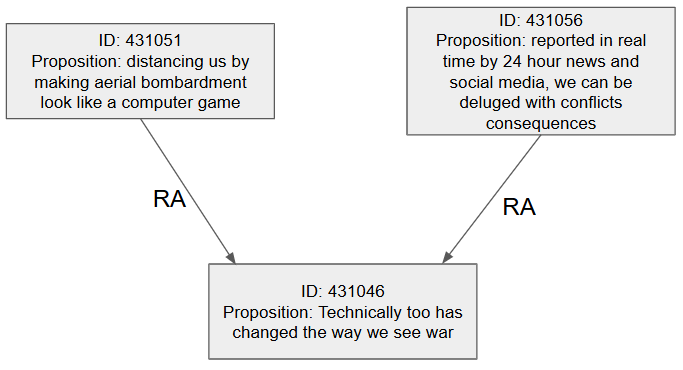
\includegraphics[width=8cm]{argument-map}
\caption{Example sub-graph. \label{fig:arg-map}}
\end{figure}

An example of the JSON structure used to store the argument data is
shown in Listing \ref{lst:arg-map}. It is also worth understanding the
link between the locution and the proposition, of which those in Listing
\ref{lst:arg-map} are good examples. The locution is exactly what is
said, and the speaker is given (in this case Matthew Taylor), whereas
the proposition can be thought of as adding a bit more context from the
surrounding dialogue. This primarily includes pronoun resolution as seen
in the first word ``she'' in the locution vs.~``Nancy Sherman'' in the
proposition.

\begin{codelisting}

\caption{Example JSON object corresponding to a Node.}\label{lst:arg-map}

\begin{Shaded}
\begin{Highlighting}[numbers=left,,]
\FunctionTok{\{}
    \DataTypeTok{"id"}\FunctionTok{:} \DecValTok{433407}\FunctionTok{,}
    \DataTypeTok{"locution"}\FunctionTok{:} \StringTok{"Matthew Taylor : she answered questions about norms and structures by talking about beliefs and campaigns and I think beliefs are different to norms and I think campaigns are different to social structures"}\FunctionTok{,}
    \DataTypeTok{"proposition"}\FunctionTok{:} \StringTok{"Nancy Sherman answered questions about norms and structures by talking about beliefs and campaigns and beliefs are different to norms and campaigns are different to social structures"}\FunctionTok{,}
    \DataTypeTok{"relations"}\FunctionTok{:} \OtherTok{[}
        \FunctionTok{\{}
            \DataTypeTok{"type"}\FunctionTok{:} \StringTok{"CA"}\FunctionTok{,}
            \DataTypeTok{"to\_node\_id"}\FunctionTok{:} \DecValTok{433393}
        \FunctionTok{\}}\OtherTok{,}
        \FunctionTok{\{}
            \DataTypeTok{"type"}\FunctionTok{:} \StringTok{"RA"}\FunctionTok{,}
            \DataTypeTok{"to\_node\_id"}\FunctionTok{:} \DecValTok{433416}
        \FunctionTok{\}}
    \OtherTok{]}\FunctionTok{,}
\FunctionTok{\}}
\end{Highlighting}
\end{Shaded}

\end{codelisting}

An array of these JSON objects can then be used to create the node pairs
required for the training and evaluation of the model.

\subsubsection{Forced Alignment}\label{forced-alignment}

\paragraph{Design}\label{design}

The audio data first had to be downsampled from 44.1kHz to the 16kHz
which is best accepted by the Wav2Vec2 transformer {[}39{]} among many
others. This can easily be achieved using FFmpeg\footnote{\url{https://ffmpeg.org/}}.
In the case of QT30, first audio had to be extracted from the video, and
collapsed into a mono track before it could be downsampled, this was
also easily achieved with FFmpeg.

Next, start and end times for each locution in the argument graph need
to be found, to allow the audio to be split per-locution (and therefore
per node). This can be achieved using Connectionist Temporal
Classification (CTC) {[}55{]} as exposed by PyTorch's forced alignment
api\footnote{\url{https://pytorch.org/audio/}}. CTC allows a model to classify
the data in a certain timestep into one of several categories (in this
case each letter) considering the data in surrounding timesteps. This
then provides the probability distribution across a set of tokens, for
each timestep (known as a frame). For a forced alignment task, these
tokens are typically each letter of the alphabet and a blank token. The
blank token is used for frames which cannot be classified as any other
token (e.g.~silence).

\begin{figure}[h]
\centering
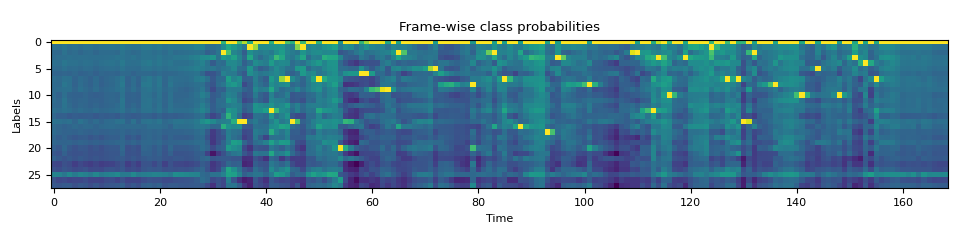
\includegraphics[width=8cm]{framewise-probs}
\caption{Example framewise probabilities. \label{fig:framewise-probs}}
\end{figure}

Figure \ref{fig:framewise-probs} (taken from the PyTorch tutorial on the
subject\footnote{\url{https://pytorch.org/audio/main/tutorials/ctc\_forced\_alignment\_api\_tutorial.html}})
shows an example of the framewise probability distribution across each
token, token 0 here is the blank token. This distribution provides the
probability (or confidence) of any particular token appearing in any
given frame. Taking simply the most probable tokens provides something
that looks like the following:
\texttt{-\ i\ -\ -\ h\ h\ a\ -\ -\ -\ d\ -}, where \texttt{-} represents
the blank token. That sequence describes the words `I had', so it can be
seen that the duplicates need to be removed, along with the blank
tokens. This is the process that would be undertaken for Automated
Speech Recognition.

When looking at forced alignment, however, the process is a bit
different since we already have a transcript. For forced alignment the
goal is to find the most probable route through the framewise
probability matrix which matches the transcript. To do this a so-called
trellis matrix can be generated. Here it is useful to envision two
`pointers', one of which represents the current frame in the audio and
the other represents the current position in the transcript. Then for
every transition between frames, consider the probability that the
position in the transcript remains the same vs.~the probability that it
moves forward one character.

We are then looking for the path across the most likely transitions,
\(k_{(t+1, j+1)}\), where \(j\) is the current location in the
transcript, and \(t\) is the current timeframe. The trellis can then be
defined as in Equation \ref{eq:trellis}.

\begin{align}
\label{eq:trellis}
k_{t+1, j+1} = \max \Bigl( & k_{(t,j)}p(t+1, c_{j+1}), \\
& k_{(t,j+1)}p(t+1, repeat) \Bigr) \nonumber
\end{align}

Where \(k\) is the trellis matrix and \(p(t, c_j)\) is the probability
of any token \(c_j\) appearing in frame \(t\), effectively referencing
the framewise probability matrix, and \(repeat\) represents the blank
token.

Once the trellis matrix is generated, an example of which is shown in
Figure \ref{fig:trellis-matrix}\footnote{\url{https://pytorch.org/audio/main/tutorials/forced\_alignment\_tutorial.html}}
where the yellow high-probability path is visually obvious, it can be
traversed using a backtracking algorithm, starting from the last token
in the transcript and following either \((c_j \rightarrow c_j)\) or
\((c_j \rightarrow c_{j-1})\) transitions, based on their probability,
until reaching the beginning of the transcript.

\begin{figure}[h]
\centering
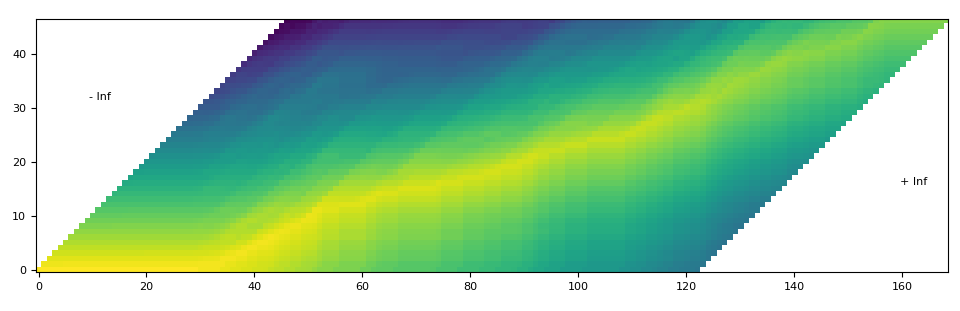
\includegraphics[width=8cm]{trellis-matrix}
\caption{Example trellis matrix where yellow shows a high probability. \label{fig:trellis-matrix}}
\end{figure}

At this point, we have start and end frame-numbers for each token, and
based on the probabilities the model has traversed, a `confidence' score
can be calculated based on the mean of the probabilities traversed, this
group of three values is known as a span (in this case a token span).
The token spans can be generated by using the PyTorch forced alignment
API, allowing the algorithm to be easily implemented and used. Finally,
the token spans can be combined into word spans based on word boundaries
in the transcript. This provides start and end frame numbers for each
word, along with a confidence score. The same process can be conducted
later to find a locution-level span with a confidence score. The frame
numbers can then be easily converted back into times in the waveform and
then split into the required segment.

\paragraph{Implementation}\label{implementation}

Initially the forced alignment of the argumentative discourse was
achieved by aligning each word in the complete transcript of the
episode, producing start and end times for each word. A search can then
be performed through these data to find the required locution. While
this technique initially produced promising results, it was not robust
enough to allow for errors in the transcripts or the crosstalk common in
debates. This problem can be seen in the fact that the trellis matrix
only allows for a single token to appear in each timeframe, which is
trivially not applicable to the real world in an argumentative context
where a lot of crosstalk (multiple speakers talking over each other)
exists.

To solve this problem, the PyTorch forced alignment API is able to take
wildcard tokens as input, therefore, each locution can be searched for
individually. To achieve this, the partial transcript used as input to
the forced aligner took the following form: \mbox{\texttt{*\ \{locution\}\ *}}.

Using this system allows the forced aligner to work well through
crosstalk (since each locution's alignments are searched for
independently of all others), and qualitatively seems to be more
resilient to errors. Error resilience is helped since errors are less
common in the locution texts as opposed to the transcripts. Using this
system also allowed for confidence scores to be collected for analysis.
In Section \ref{sec:datasets-audio} general analysis across all corpora
is performed, with corpus specific analysis in the relevant section.

\subsubsection{Audio Data}\label{sec:datasets-audio}

Figure \ref{fig:complete-confidence} shows the distribution of
confidence scores across both the QT30 corpus and all Moral Maze
corpora. This distribution shows that the system can relatively
confidently align the majority of locutions, with only approximately 8\%
of locutions with a confidence score less than \(0.50\).

\begin{figure}[h!]
\centering
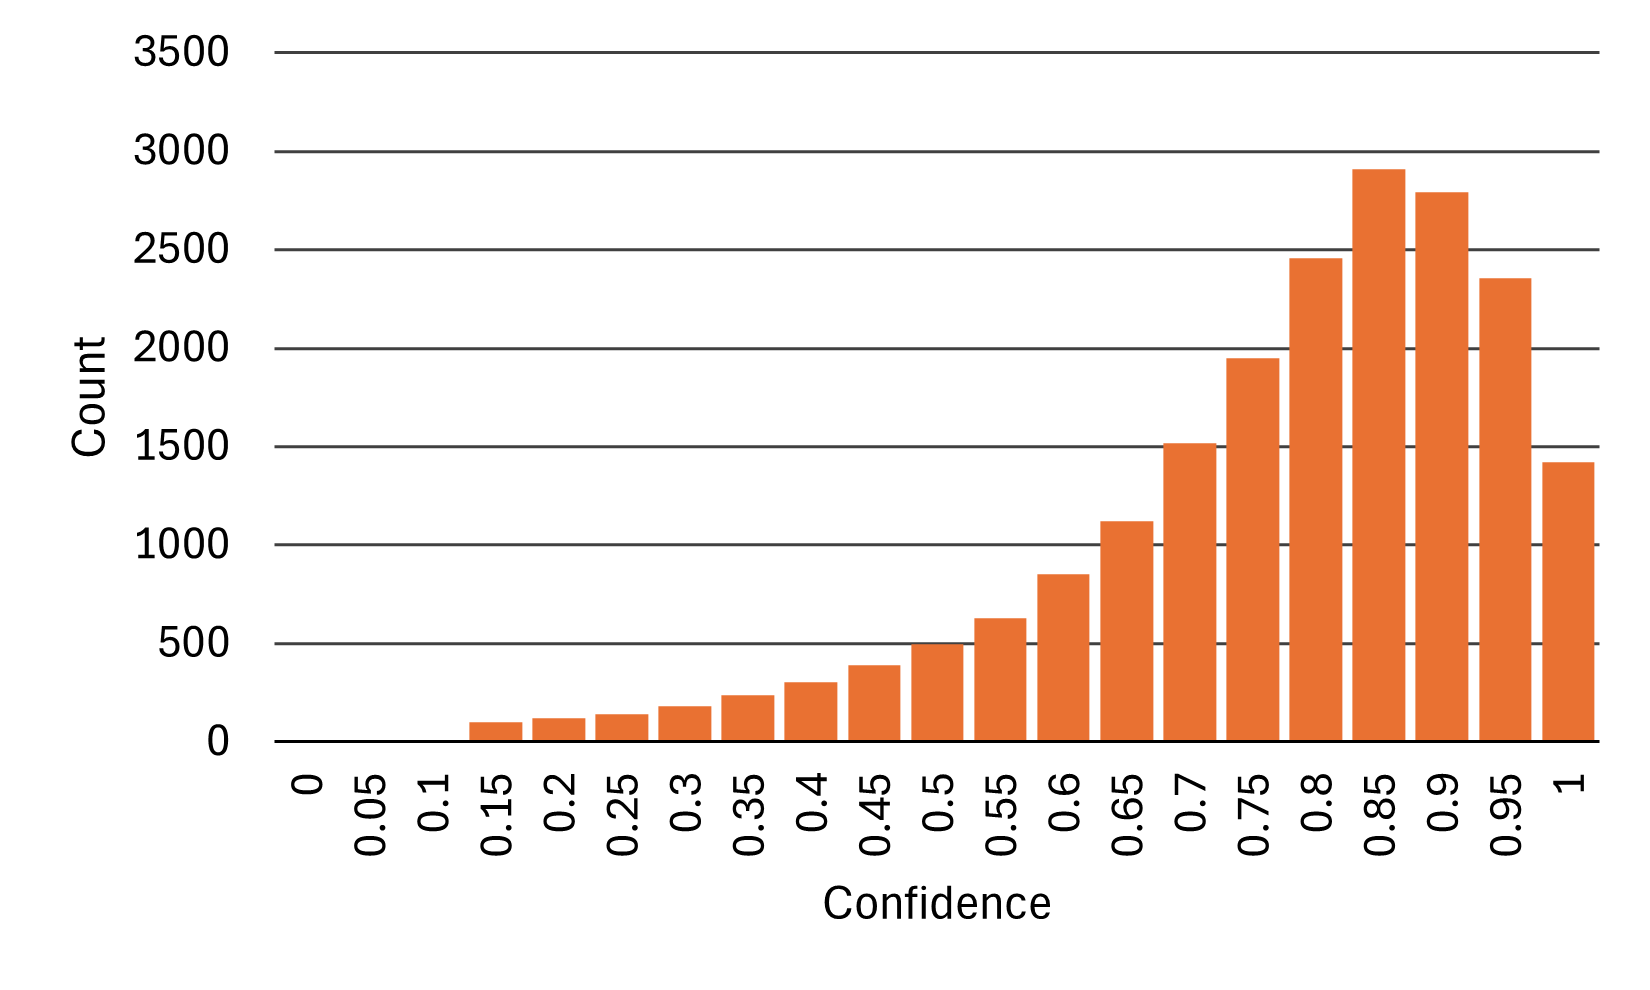
\includegraphics[width=8cm]{complete-confidence}
\caption{Confidence distribution across all corpora. \label{fig:complete-confidence}}
\end{figure}

In order to further analyse the performance of this system, locutions
were selected at random and qualitatively analysed. Throughout this
process, all locutions appeared correct, however, it was very
challenging to manually determine the accuracy of the system on
locutions with confidence scores \(<0.2\) due to high amounts of
crosstalk or other acoustic artefacts. This shows that this method of
aligning locutions with their corresponding audio is accurate for the
purposes of this project, as long as the confidence scores are taken
into account. However, these confidence scores should not be mistaken
for a `probability of being correct'.

The distribution of lengths for each audio clip was also analysed in
order to ensure the models are being provided with enough data. The
primary statistics are shown in Table \ref{tbl:audio-complete}. These
data shows that the majority of locutions are shorter than 8 seconds
(approximately 120,000 samples at the sampling rate of 16kHz). In total,
across both corpora, there is over 24 hours of argumentative audio, out
of over 36 hours of total audio processed. The relevant data for the
specific corpora are detailed in the relevant section.

\begin{table}[h]
\centering
\caption{Audio data for locutions across all corpora.\label{tbl:audio-complete}}
\begin{tabular}{|l|ll|}
\hline
Quantity        & Length (s) & No. of Samples \\ \hline
Mean            & 3.9        & 62,000         \\
75th Percentile & 5.1        & 81,000         \\
90th Percentile & 7.7        & 120,000        \\
Maximum         & 31         & 490,000        \\ \hline
\end{tabular}
\end{table}

Next, a comparison can be made between the sizes of the datasets
presented here (QT30-MM and Moral Maze) when compared to previous work
in ARI and other AM subtasks. Table \ref{tbl:mm-comparison} compares the
M-Arg {[}7{]}, VivesDebate-Speech {[}5{]}, UKDebates {[}56{]}, MM-USED
{[}4{]} and MM-USED-fallacy {[}57{]}. As far as could be ascertained,
QT30-MM is by far the biggest multimodal ARI dataset created
to date with 20 hours of argumentative audio and although the Moral Maze
corpus only contains 5 hours of argumentative audio, it is the only
cross-domain corpus. It should be noted, however, that the MM-USED and MM-USED-fallacy are larger argument mining datasets but only contain annotations for ACC or fallacy detection.

\begin{table}[h]
\centering
\caption{Comparison between different multimodal argument mining datasets. Lengths are in hours. *dataset lengths were not reported by initial authors so are derived from downloaded audio data. \label{tbl:mm-comparison}}
\begin{tabular}{|l|l|l|}
\hline
Dataset            & Task              & Length \\ \hline
M-Arg              & ARI               & 7              \\
VivesDebate-Speech & ARI, ASD          & 12             \\
UKDebates          & Claim Detection   & 2              \\
MM-USED            & ACC          & 43*           \\
MM-USED-fallacy    & Fallacy Detection & 37*           \\ \hline
QT30-MM            & ARI               & 20             \\
Moral Maze         & ARI               & 5              \\ \hline
\end{tabular}
\end{table}

\subsubsection{ADU Pair Creation}\label{sec:pair-creation}

Finally, a set of node pairs and their relations can be generated in
order to train a neural network. For related nodes this can be done
trivially in that for each relation, the corresponding pair of nodes can
be added to the set. When sampling unrelated nodes, however, things are
more complex.

It has also been shown that how unrelated node pairs are sampled is very
relevant to the model's performance {[}51{]}. For this reason, it is
also useful to provide a comparison between the different methods in a
multimodal context. Since a short context is defined as being within an
episode, the sampling strategies are only relevant for QT30, all Moral
Maze episodes are simply undersampled. The following methods are
compared:

\begin{itemize}
\tightlist
\item
  \textbf{Undersampling (US)} is the simplest method. The set of all
  possible pairs is created and then randomly undersampled to the number
  of inference/support relations.
\item
  \textbf{Long Context Sampling (LCS)} samples unrelated nodes such that
  each node comes from a different episode with the result that they are
  `far apart' in the discourse, this often takes the form of a different
  topic and such the task is slightly easier than the other methods.
  This list can then be randomly undersampled to the number of
  inference/support relations.
\item
  \textbf{Short Context Sampling (SCS)} samples unrelated such that each
  node comes from the same episode so they are `close together' in the
  discourse meaning that they often involve the same topic with the
  result that the task is slightly harder than other methods. This set
  is then randomly undersampled to the number of inference/support
  relations.
\end{itemize}

\subsection{QT30}\label{qt30}

The QT30 argument corpus {[}17{]} contains transcripts and argument
annotations for 30 episodes of the BBC's Question Time, a series of
televised topical debates across the United Kingdom. All episodes aired
in 2020 and 2021. The corpus is split into 30 subcorpora, each spanning
a single episode. This creates a large corpus with almost 20k locutions.
What follows is an analysis of the corpus and how audio data were added.

Table \ref{tbl:qt-rel} shows the distribution of each type of relation
across QT30. Inference and Rephrase relations make up a total of
\(91.5\%\) of the dataset, with Conflict relations being significantly
less common, only making up \(8.5\%\) of the dataset. It is obvious that
this is an unbalanced dataset, which will have to be considered during
training.

\begin{table}[h]
\centering
\caption{Distribution of propositional relations in QT30. \label{tbl:qt-rel}}
\begin{tabular}{|l|ll|}
\hline
Relation Type & Count & Proportion (\%) \\ \hline
Inference     & 5,761       & 51.4\%    \\
Conflict      & 947         & 8.5\%     \\
Rephrase      & 4,496       & 40.1\%    \\ \hline
Total         & 11,204      & 100\%     \\ \hline
\end{tabular}
\end{table}

Figure \ref{fig:qt30-confidence-box} shows a box plot of the mean
confidence values across each episode. This plot shows two outliers
corresponding to the 22July2021 episode (with mean confidence 0.44) and
the 30September2021 episode (with mean confidence 0.24). Manually
analysing samples in these episodes indicates a high error rate in the
alignment of locutions. Because of this high error rate, it was decided
to exclude these episodes from the corpus used for training. The rest of
the episodes from QT30 will form its multimodal subcorpus (QT30-MM)
where QT30-MM has a mean confidence score of 0.75 with a standard
deviation of 0.17.

\begin{figure}[h]
\centering
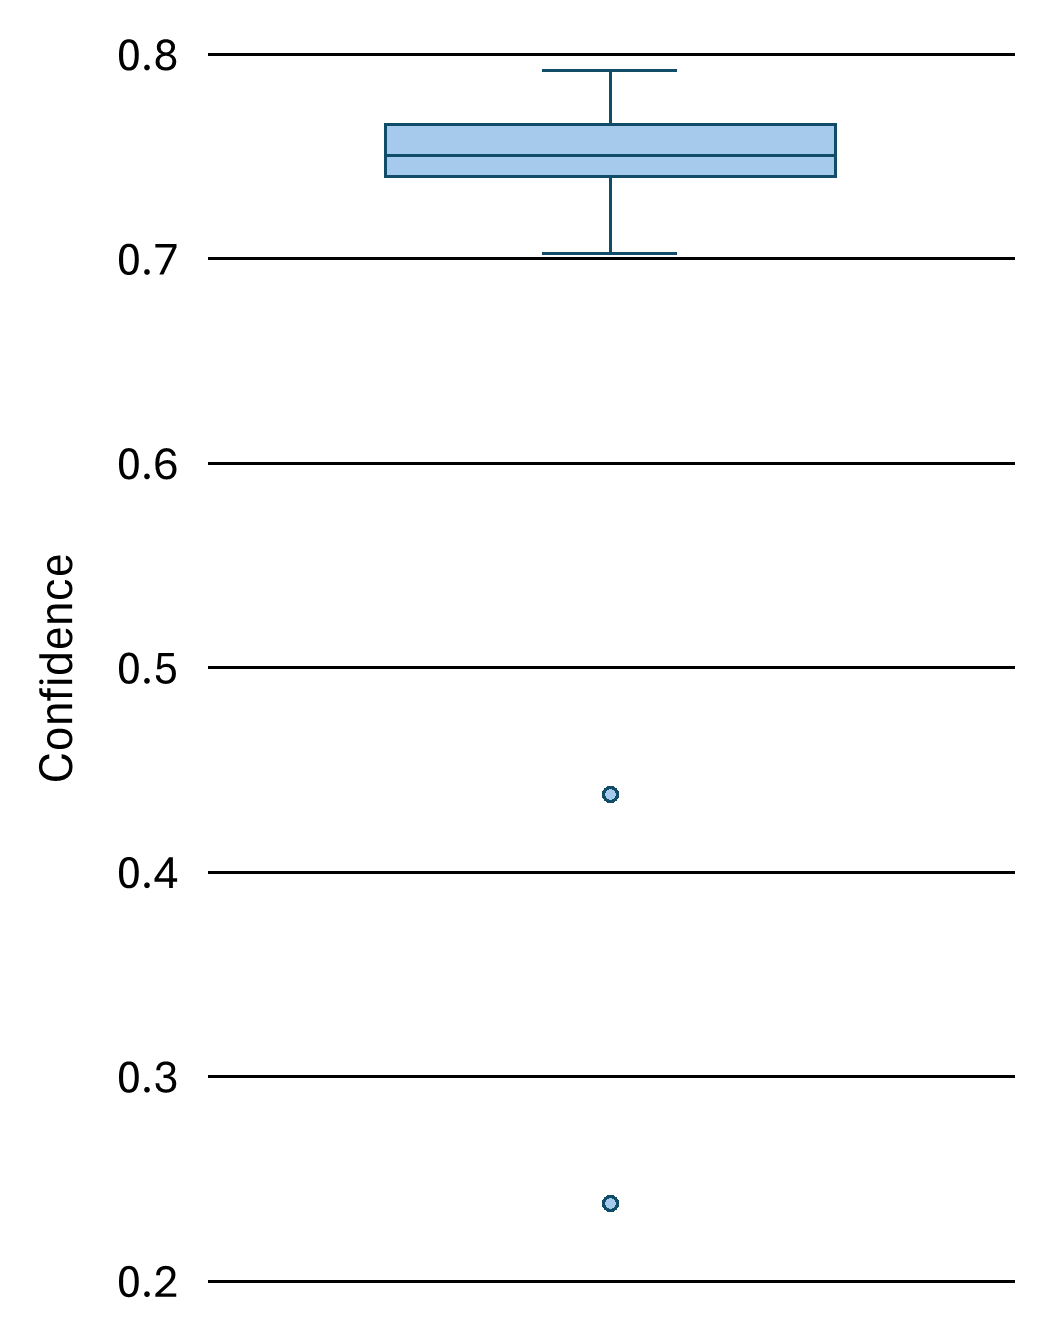
\includegraphics[height=8cm]{confidence-box}
\caption{Box plot of episodic confidence values across QT30. \label{fig:qt30-confidence-box}}
\end{figure}

As can be seen in Figure \ref{fig:qt30-mm-confidence} the distribution
of confidence scores closely matches that shown in Figure
\ref{fig:complete-confidence}. This still indicates that the audio
alignments are calculated with high accuracy.

\begin{figure}[h]
\centering
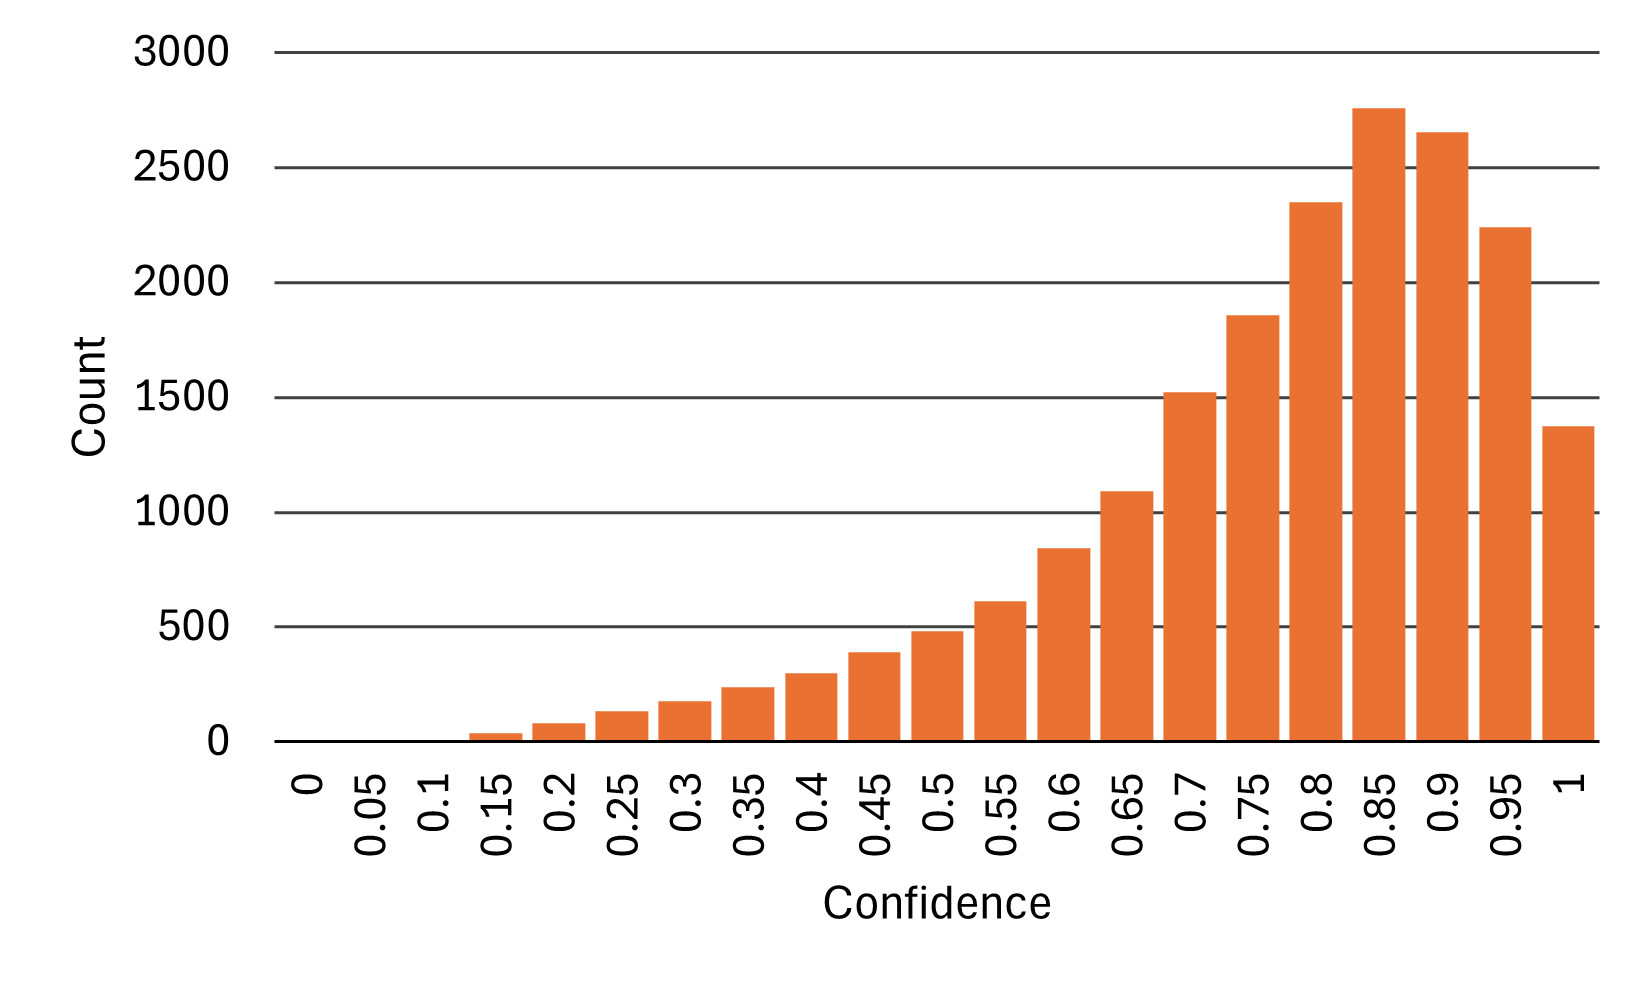
\includegraphics[width=8cm]{qt30-mm-confidence}
\caption{Confidence distribution across QT30-MM. \label{fig:qt30-mm-confidence}}
\end{figure}

Table \ref{tbl:qt-mm-rel-no} shows the distribution of relations after
sampling unrelated nodes, this process increases the dataset size to a
total of almost 17k samples. When comparing QT30 to QT30-MM the total
number of relations only drops from 11,204 in QT30 to 11,156 in QT30-MM
(only losing 48 relations), however, the quality of audio alignment does
increase.

\begin{table}[h]
\centering
\caption{Distribution of propositional relations after sampling non-related nodes. \label{tbl:qt-mm-rel-no}}
\begin{tabular}{|l|ll|}
\hline
Relation Type & Count  & Proportion (\%) \\ \hline
None          & 5,470  & 34\%            \\
Inference     & 5,470  & 34\%            \\
Conflict      & 937    & 6\%             \\
Rephrase      & 4,479  & 27\%            \\ \hline
Total         & 16,896 & 100\%           \\ \hline
\end{tabular}
\end{table}

The audio data contained within the dataset can also be analysed as
shown in Table \ref{tbl:audio-data-qt}. Generally the values are very
similar to those shown in Table \ref{tbl:audio-complete}. The QT30-MM
dataset contains almost 20 hours of argumentative audio taken from
approximately 29.5 hours of total audio. This makes the QT30-MM corpus
the largest multimodal ARI dataset currently available.

\begin{table}[h]
\centering
\caption{Audio data for locutions across QT30-MM.\label{tbl:audio-data-qt}}
\begin{tabular}{|l|ll|}
\hline
Quantity        & Length (s) & No. of Samples \\ \hline
Mean            & 3.8        & 60,000         \\
75th Percentile & 5.0        & 79,000         \\
90th Percentile & 7.5        & 120,000        \\
Maximum         & 30         & 470,000        \\ \hline
\end{tabular}
\end{table}

\subsection{Moral Maze}\label{moral-maze}

Similar to Question Time, the BBC's Moral Maze is a series of radio
broadcast debates, with each episode focusing on a certain topic.
Several episodes of the Moral Maze have been annotated with IAT and AIF
and also made available on AIFdb. Of these episodes, eight were chosen
from different fields. It is therefore these eight episodes, released
from 2012 to 2019, which this project considers. Each episode focuses on
a very different domain which allows for a robust, cross-domain analysis
of any models trained on another corpus (e.g.~QT30). The Moral Maze
corpus contains data from eight different episodes: Banking (B), Empire
(E), Money (M), Problem (P), Syria (S), Green Belt (G), Hypocrisy (H)
and Welfare (W). Each episode consists of a debate focusing on a
different topic, and hence has a different distribution of classes.

Table \ref{tbl:moral-rel-no} shows the distribution of propositional
relations across the Moral Maze corpus, after unrelated pairs have been
sampled. Comparing the corpus to QT30, a significantly lower proportion
of the corpus is made up of Rephrase relations. It is possible that the
differing formats of the debates has an impact here.

\begin{table*}[t]
\centering
\caption{Distribution of propositional relations across the Moral Maze corpus. \label{tbl:moral-rel-no}}
\begin{tabular}{|l|llll|l|}
\hline
Subcorpus \textbackslash  Relation Type & None         & Inference    & Conflict  & Rephrase  & Total \\ \hline
B             & 132 (45\%)   & 132 (45\%)   & 24 (8\%)  & 3 (1\%)   & 291   \\
E             & 151 (41\%)   & 151 (41\%)   & 39 (11\%) & 25 (7\%)  & 366   \\
M             & 255 (43\%)   & 255 (43\%)   & 29 (5\%)  & 58 (10\%) & 597   \\
P             & 236 (42\%)   & 236 (42\%)   & 40 (7\%)  & 45 (8\%)  & 557   \\
S             & 181 (42\%)   & 181 (42\%)   & 63 (14\%) & 10 (2\%)  & 435   \\
G             & 301 (41\%)   & 301 (41\%)   & 46 (6\%)  & 93 (13\%) & 741   \\
H             & 207 (43\%)   & 207 (43\%)   & 23 (5\%)  & 43 (9\%)  & 480   \\
W             & 211 (40\%)   & 211 (40\%)   & 59 (11\%)  & 43 (8\%)  & 524   \\ \hline
Total         & 1,674 (42\%) & 1,674 (42\%) & 323 (8\%) & 320 (8\%) & 3,991 \\ \hline
\end{tabular}
\end{table*}

Figure \ref{fig:mm-confidence-box} shows a box plot of the mean
confidence scores for each subcorpus of Moral Maze. Generally the
results match what is expected and are similar to those in QT30 although
there are no outliers and therefore no episodes were omitted.

\begin{figure}[h]
\centering
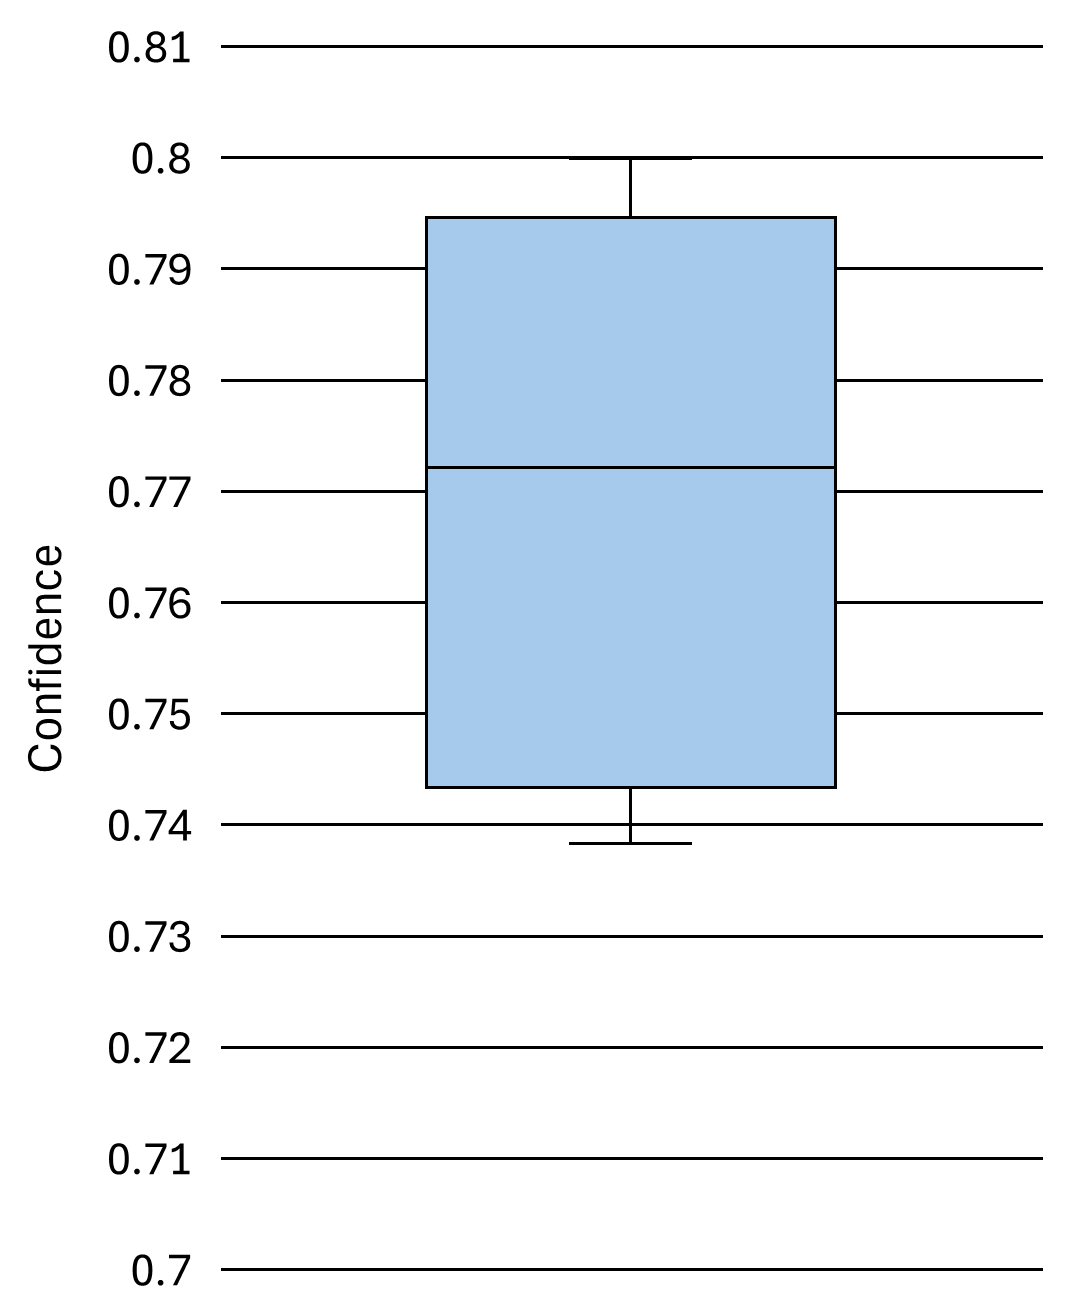
\includegraphics[height=8cm]{mm-confidence-box}
\caption{Per-subcorpus mean of confidence scores for each Moral Maze episode. \label{fig:mm-confidence-box}}
\end{figure}

In Figure \ref{fig:moral-confidence} the distribution of audio alignment
confidence scores across all Moral Maze episodes can be seen. This
follows the expected pattern as shown in Figures
\ref{fig:complete-confidence} and \ref{fig:qt30-mm-confidence}.

\begin{figure}[h]
\centering
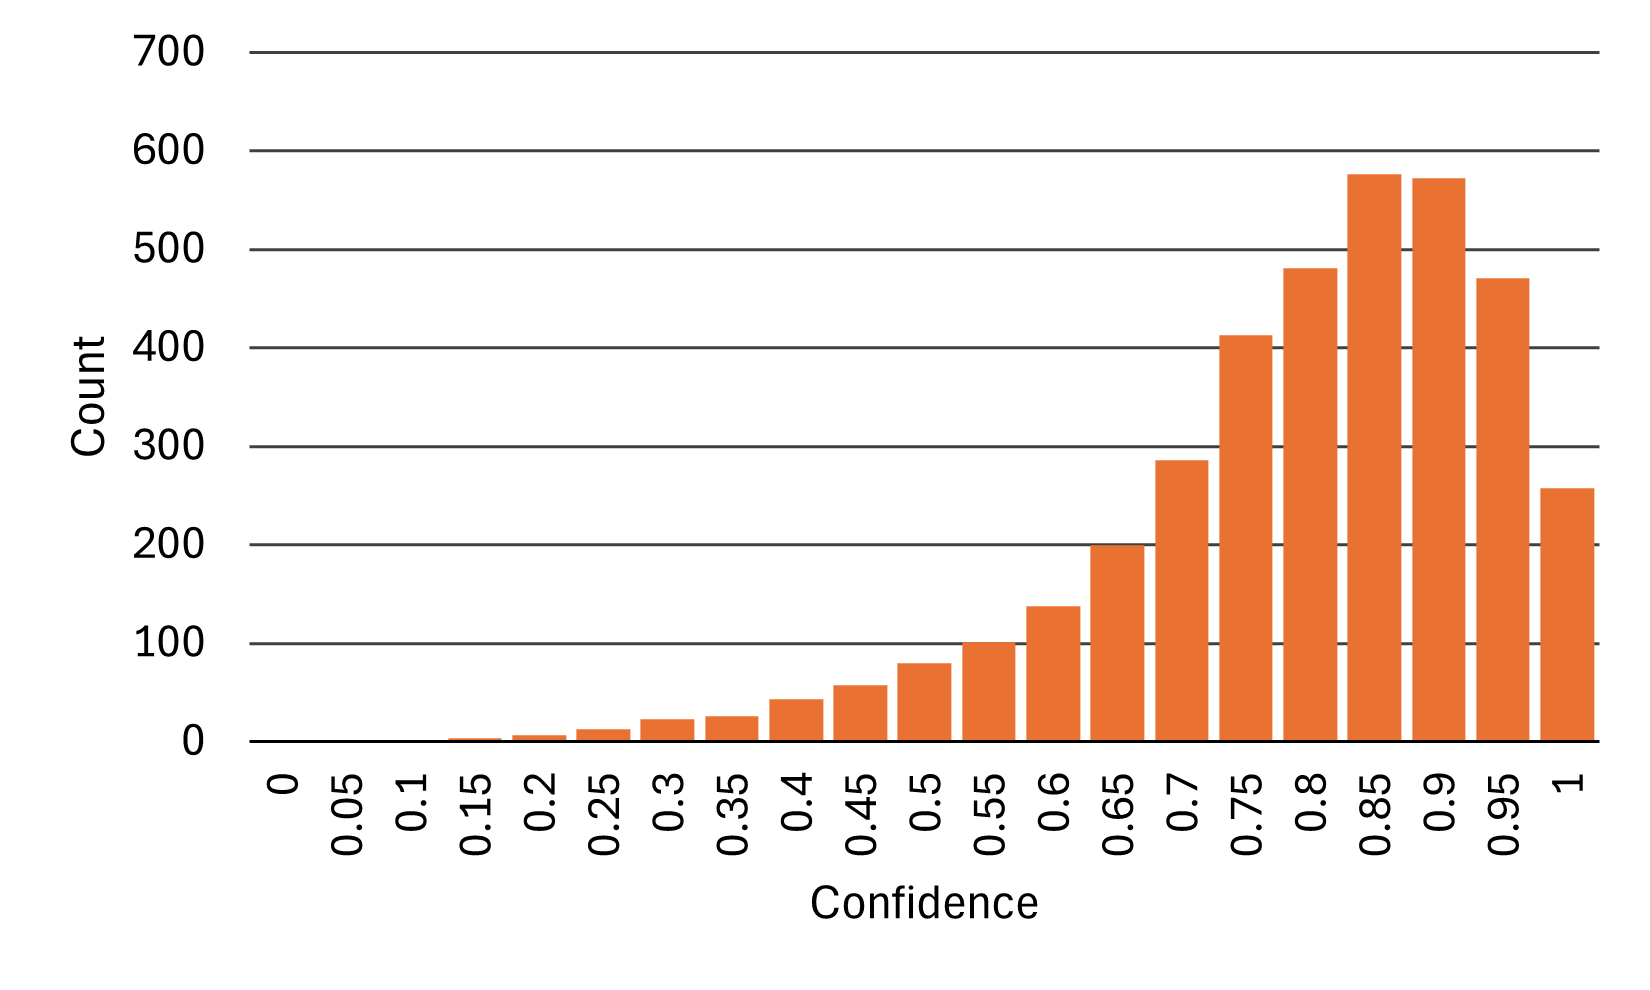
\includegraphics[width=8cm]{moral-confidence}
\caption{Confidence distribution across all Moral Maze subcorpora. \label{fig:moral-confidence}}
\end{figure}

Table \ref{tbl:audio-data-mm} shows the statistics for the audio part of
the combined Moral Maze corpus. Generally the locutions seem to be a bit
longer in the Moral Maze when compared to QT30. The Moral Maze combined
corpus contains almost 5 hours of argumentative audio taken from
approximately 6.5 hours of total audio.

\begin{table}[h]
\centering
\caption{Audio data for locutions across Moral Maze.\label{tbl:audio-data-mm}}
\begin{tabular}{|l|ll|}
\hline
Quantity        & Length (s) & No. of Samples \\ \hline
Mean            & 4.4        & 70,000         \\
75th Percentile & 5.8        & 94,000         \\
90th Percentile & 9.0        & 140,000        \\
Maximum         & 31         & 490,000        \\ \hline
\end{tabular}
\end{table}

\section{Models}\label{sec:models}

This section descries the model architectures that are evaluated in this
project. Since the models will be aimed at a sequence pair
classification task, there is a distinction between when the data from
each sequence is combined (which can be termed sequence fusion) and when
the data from each modality is combined (which can be termed multimodal
fusion). The following subsections define the different approaches
evaluated for each of these stages.

In previous work it has been shown that the RoBERTa models perform
better than other pretrained transformers on the task of ARI {[}15{]}.
To encode the text data, the RoBERTa-base model is used, with 12 encoder
layers, each with 12 attention heads and a hidden size of 768, resulting
in 110M total parameters\footnote{\url{https://huggingface.co/FacebookAI/roberta-base}}.
Wav2Vec 2.0 is also used in many audio processing \mbox{tasks {[}3, 6{]}}
and therefore is used to encode the audio data. To ensure both models
output the same hidden size, the wav2vec2-base model is used with 95M
total parameters\footnote{\url{https://huggingface.co/facebook/wav2vec2-base-960h}}.
The wav2vec2 model used is fine-tuned on 960 hours of librispeech for
automatic speech recognition. Once the data have been encoded, it can be
fed into the classification head to output a final prediction.

The classification head used for most models is a simple linear
projection from the hidden vector down to the required number of
classes. The best performing model on ARI as proposed in MAMKit {[}6{]}
(MM-RoBERTa) is also evaluated. Their model uses the fusion architecture
described in Figure \ref{fig:model-diag-late} but with a 3 layer
Multilayer Perceptron (MLP) model as the classification head. They also
only train the classification head, without training the text or audio
encoders.

\subsection{Sequence Fusion}\label{sec:seq-fusion}

In most text-processing approaches the data from each sequence is
combined at the text level using special tokens defined in the encoder's
\mbox{tokeniser {[}16, 47, 48{]}}. For this project, this approach
is termed early sequence fusion. To achieve this, the input sequences
can be delimited by a separator token, and the entire sequence wrapped
in the start of sequence (SOS) and end of sequence (EOS) tokens. An
example using the RoBERTa tokeniser takes the following form:

\begin{quote}
\texttt{\textless{}s\textgreater{}\ {[}sequence\ 1{]}\ \textless{}/s\textgreater{}\ {[}sequence\ 2{]}\ \textless{}/s\textgreater{}}
\end{quote}

Here the \texttt{\textless{}s\textgreater{}} token corresponds to the
SOS, and \texttt{\textless{}/s\textgreater{}} does the job of both the
separator token and the EOS token.

Next the audio data can be considered. As far as was found, there is no
existing literature on how early sequence fusion could function for
audio models. Therefore, it was decided to delineate each audio sequence
by a certain amount of silence. The exact amount of silence could be
adjusted as a training hyperparameter and was eventually set to 5
seconds.

Figure \ref{fig:model-diag-early} shows an example of a model
architecture using this late fusion technique, text related steps are
shown in purple and audio related steps are shown in green. RoBERTa and
Wav2Vec2 are simply used as examples and could be substituted for other
models.

\begin{figure}[h]
\centering
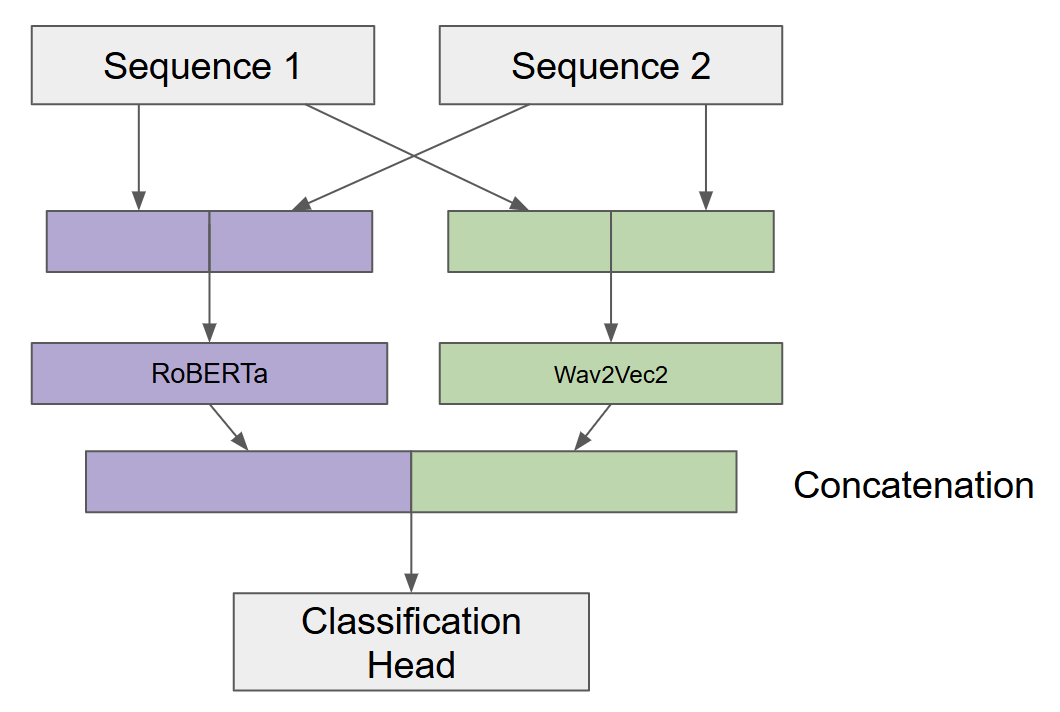
\includegraphics[width=8cm]{model-diag-early}
\caption{Model diagram with early sequence and late multimodal fusion. Purple denotes textual data and green denotes acoustic data.\label{fig:model-diag-early}}
\end{figure}

Mestre \emph{et al.} {[}7{]} and Mancini \emph{et al.} {[}6{]} approach
the problem differently. They first put each sequence through the text
encoder independently, before fusing the outputs and feeding the
combined encodings into the classification head. While concatenation is
the only fusion method examined for this sequence fusion technique,
others (such as an element-wise product or cross-attention) could be
used. This approach extends much more easily to the audio modality,
since the audio encodings can be combined in the same way as the text
encodings. This approach to fusing the data in each sequence can be
termed late sequence fusion. Figure \ref{fig:model-diag-late} shows an
example of a model architecture using late sequence fusion, text
processing steps and data are shown in purple and audio-related steps
are shown in green.

\begin{figure}[h]
\centering
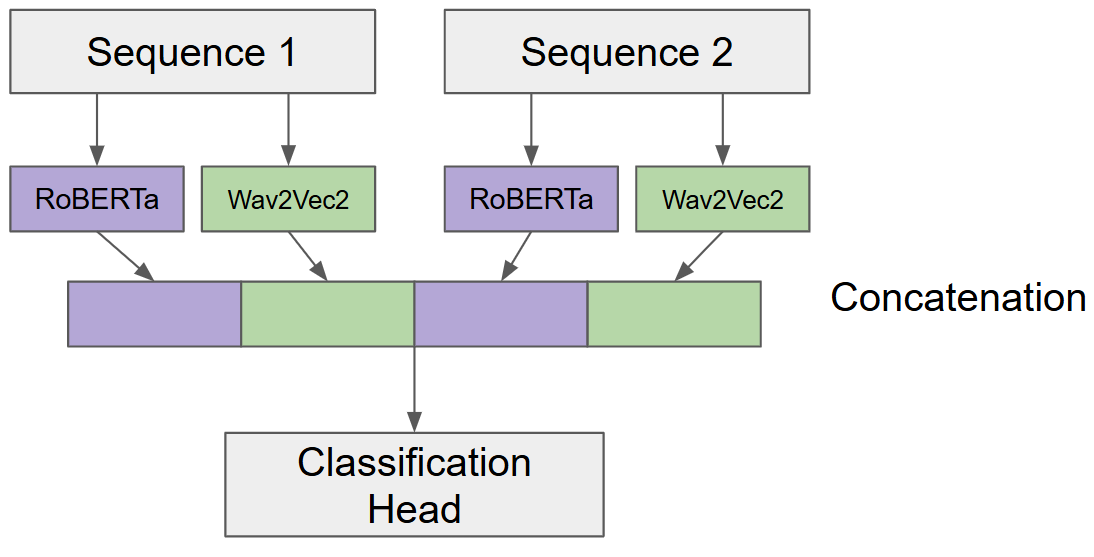
\includegraphics[width=8cm]{model-diag-late}
\caption{Model diagram with late concatenation sequence and multimodal fusion. Purple denotes textual data and green denotes acoustic data.\label{fig:model-diag-late}}
\end{figure}

\subsection{Multimodal Fusion}\label{sec:mm-fusion}

Multimodal fusion decribes the method by which the text and audio data
are combined. As detailed in Section \ref{sec:background-ml}, fusion
techniques can be split into two major categories: early and late
fusion. This project only evaluates late fusion techniques due to their
ease of development and the applicability of pre-trained models. The
following techniques are evaluated:

\begin{itemize}
\tightlist
\item
  \textbf{Concatenation} where the pooled encodings for each modality
  are simply concatenated before being fed into the classification head.
\item
  \textbf{Elementwise-product} (otherwise known as a Hadamard product)
  takes the product of each element in the pooled encodings for each
  modality.
\item
  \textbf{Crossmodal Attention} (CA) is similar to the self-attention
  mechanism found in transformers, however, the queries are taken from a
  different modality when compared to the keys and values. To compute
  crossmodal attention features, the query and key matrices are
  multiplied and then put through a softmax. This is then multiplied
  with the value matrix and the result can then be pooled using an
  arithmetic mean. For the purposes of this project, the CA module is
  labelled based on the modality from which the query matrix is derived
  (e.g.~a \texttt{CA\_Text} module derives the query matrix from the
  text encodings and the key and value matrices from the audio
  encodings). This is shown in Figure \ref{fig:crossmodal-attention}.
\end{itemize}

\begin{figure*}[t!]
\centering
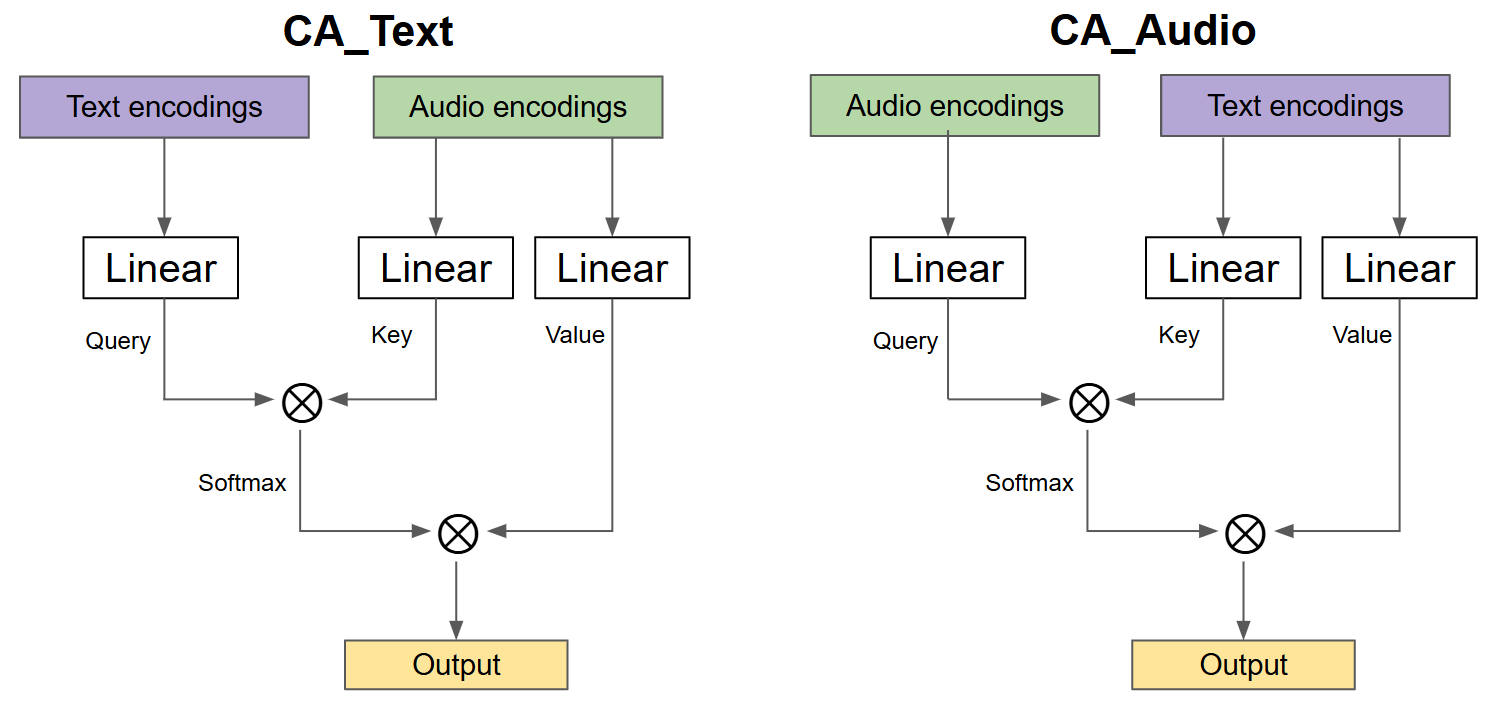
\includegraphics[width=16cm]{crossmodal-attention}
\caption{Crossmodal attention system with both text and audio queries. $\otimes$ is used to denote matrix multiplication.\label{fig:crossmodal-attention}}
\end{figure*}

Listing \ref{lst:crossattention} shows how a crossmodal attention
mechanism can be implemented into a PyTorch module. The code is
contained within the forward method of a PyTorch module, where
\texttt{self.query\_proj}, \texttt{self.key\_proj} and
\texttt{self.value\_proj} are the linear projections for the queries,
keys and values respectively. \texttt{torch.bmm} refers to a matrix
multiplication and \texttt{F.softmax} is a mathematical function to
ensure all values (across the requested dimension) lie in the range
\([0,1]\) and sum to 1, the softmax function for a vector \(\mathbf{x}\)
is given in Equation \ref{eq:softmax}.

\begin{equation} \text{Softmax}(x_i) = \frac{\exp(x_i)}{\sum_j \exp(x_j)} \label{eq:softmax}\end{equation}

\begin{codelisting}[H]

\caption{PyTorch forward method for a crossmodal attention mechanism.}\label{lst:crossattention}

\begin{Shaded}
\begin{Highlighting}[numbers=left,,]
\CommentTok{\# project query features}
\NormalTok{queries }\OperatorTok{=} \VariableTok{self}\NormalTok{.query\_proj(query\_modality)}

\CommentTok{\# project kv features}
\NormalTok{keys }\OperatorTok{=} \VariableTok{self}\NormalTok{.key\_proj(kv\_modality)}
\NormalTok{values }\OperatorTok{=} \VariableTok{self}\NormalTok{.value\_proj(kv\_modality)}

\CommentTok{\# compute attention scores}
\NormalTok{attn\_scores }\OperatorTok{=}\NormalTok{ torch.bmm(queries, keys.transpose(}\DecValTok{1}\NormalTok{, }\DecValTok{2}\NormalTok{))}
\NormalTok{attn\_probs }\OperatorTok{=}\NormalTok{ F.softmax(attn\_scores, dim}\OperatorTok{={-}}\DecValTok{1}\NormalTok{)}

\CommentTok{\# compute and return cross modal features}
\ControlFlowTok{return}\NormalTok{ torch.bmm(attn\_probs, values)}
\end{Highlighting}
\end{Shaded}

\end{codelisting}

\section{Results}\label{results}

\subsection{Experimental Setup}\label{sec:exp-setup}

To provide a comparable set of results, all experiments were run using
the same hyperparameters. Each model was trained on a single Nvidia RTX
4070 Super for 15 epochs with a batch size of 32 using a weighted
cross-entropy loss and the AdamW optimiser {[}58{]} initialised with a
learning rate of \(10^{-5}\), a linear learning rate scheduler and 10\%
of training used as warm-up steps. The cross-entropy weights were
calculated as in Equation \ref{eq:weight}, where \(\mathbf{c}\) is a
vector containing the number of samples in each class, and
\(\mathbf{w}\) is a vector containing the relevant cross-entropy weight.

\begin{equation} w_i = \frac{\max(\mathbf{c})}{c_i} \label{eq:weight}\end{equation}

Using these hyperparameters was found to provide a good balance between
model performance and training time on the hardware used with the
weighted cross-entropy loss.

In order to evaluate the models, the following metrics are reported:
macro-averaged F1 score, precision and recall. These are all described
for each class in Equations \ref{eq:f1}, \ref{eq:precision} and
\ref{eq:recall} where \(TP\) is the number of true positives, \(FP\) is
the number of false positives and \(FN\) is the number of false
negatives. The arithmetic mean can then be taken for each class to
provide a holistic overview of the model's performance.

\begin{equation} F1 = \frac{2TP}{2TP + FP + FN} \label{eq:f1}\end{equation}

\begin{equation} \text{Precision} = \frac{TP}{TP + FP} \label{eq:precision}\end{equation}

\begin{equation} \text{Recall} = \frac{TP}{TP + FN} \label{eq:recall}\end{equation}

Generally the macro-averaged F1 score is the standard to evaluate a
multi-class classification problem, including ARI systems {[}6,
15, 51{]}, where only a single metric is reported, it will be a
macro-averaged F1 score for this reason.

To provide a useful evaluation and simulate a real-world environment,
the QT30-MM dataset is split into three splits: train, validation and
test. 70\% of the data is allocated for training, 10\% for validation
and the remaining 20\% for testing. The model is evaluated on the
validation split after every training epoch, the best performing model,
based on macro-F1, is then chosen to be tested on the testing split, the
metrics are then calculated and reported in the following sections.

After training, each model is then evaluated on the complete dataset for
each Moral Maze episode (Banking, Empire, Money, Problem, Syria, Green
Belt, Hypocrisy and Welfare) and each metric calculated to provide an
overview of the cross-domain performance of the model.

In order to evaluate the different methods to sample unrelated arguments
as described in Section \ref{sec:pair-creation}. Models are trained on
SCS, US and LCS, the validation dataset is sampled identically to the
training set, and tested, both in-domain and cross-domain on SCS. This
is used because of its description as a more realistic problem {[}51{]}.
All code used for the experiments can be found on GitHub\footnote{\url{https://github.com/Syn-Tax/cross-domain-am}}.

\subsection{In-Domain}\label{sec:res-id}

Results are reported for both the 3-class problem (considering support,
attack and no relation) and the 4-class problem (considering RA, CA, MA
and NO). First results are considered when evaluating in-domain, i.e.~on
the test set of the QT30-MM dataset. Only macro-f1 scores are reported
here, precision and recall scores are also reported in Appendix
\ref{app:results}.

\subsubsection{The 4-Class Problem}\label{sec:id-4class}

Table \ref{tbl:results-early-4class} shows the macro-f1 scores of each
model using RoBERTa-base as the text encoder and Wav2Vec2-base as the
audio encoder. All that is shown are the results for models performing
early sequence fusion across different NO-sampling strategies. In the
4-class problem it does not seem that the addition of acoustic features
makes much if any difference to the performance of the model on the ARI
task. This result has also been found by others {[}7{]}.

In some runs, the audio only models do not learn above the performance
of the random baseline, it is unclear why this occurs but it appears to
be random. Comparing the NO-sampling strategies there does not seem to
make an appreciable difference when tested on SCS. Because SCS is
considered a much more challenging task {[}51{]} it would not be
expected that models trained on LCS or US would perform nearly as well
as those trained on SCS, however, this does not seem to be the case. The
result of this experiment implies that regardless of the sampling
strategy the model is able to acquire the same knowledge and would
likely perform similarly in a real-world setting, it is simply that SCS
evaluations are harder than US evaluations which in turn are harder than
LCS evaluations.

\begin{table}[h]
\centering
\caption{Macro-F1 scores for early sequence fusion models on the 4-class problem. Highest results in each column are shown in bold.\label{tbl:results-early-4class}}
\begin{tabular}{|l|lll|}
\hline
Model         & SCS          & LCS          & US          \\ \hline
Text Only     & \textbf{.58} & \textbf{.59} & \textbf{.59} \\
Audio Only    & .43          & .41          & .20          \\ \hline
Concatenation & \textbf{.58} & .57          & .58          \\
Product       & .56          & .57          & .58          \\
CA Text       & .57          & .46          & .57          \\
CA Audio      & \textbf{.58} & .57          & .57          \\ \hline
Random        & .22          & .23          & .24          \\
Majority      & .14          & .14          & .14          \\ \hline
\end{tabular}
\end{table}

The different sequence fusion techniques are also compared in Table
\ref{tbl:results-seq-4class}. Here it can be seen that early sequence
fusion techniques outperform late fusion techniques by approximately
50\% for both text only and audio only with concatenation showing
greater improvement at approximately 60\%. This increase in performance
is likely attributed to the fact that when the sequences are fused
before the attention mechanisms are applied the model is able to make
the long-range dependencies across sequences. This comes in contrast to
the fact that the model is unable to make any dependencies
cross-sequence when they are fused after the attention mechanisms are
applied.

\begin{table}[h]
\centering
\caption{Macro-F1 scores across sequence fusion types when trained on SCS on the 4-class problem. \label{tbl:results-seq-4class}}
\begin{tabular}{|l|ll|}
\hline
Model         & Early       & Late      \\ \hline
Text Only     & .58         & .36       \\
Audio Only    & .43         & .28       \\
Concatenation & .58         & .38       \\ \hline
Random        & \multicolumn{2}{c|}{.22} \\
Majority      & \multicolumn{2}{c|}{.14} \\ \hline
\end{tabular}
\end{table}

What follows is a more in-depth discussion of the results with the hope
that it will yield some understanding of the models' limitations and how
they could be improved. In order to do this the text only model trained
on SCS is explored in detail, however, the conclusions were found to
hold on other models. A good place to begin here is by analysing the
class F1 distribution, here F1 scores are reported for each of the four
classes (NO, RA, CA and MA). As can be seen in Table
\ref{tbl:class-f1-4class} the model performs significantly worse when
shown a conflict relation as opposed to the other possible classes. It
is possible that this is due to the significant class imbalance present
in almost all ARI datasets as discussed in Section \ref{sec:datasets}.

\begin{table}[h]
\centering
\caption{Class F1 distribution for text only SCS model.\label{tbl:class-f1-4class}}
\begin{tabular}{|llll|}
\hline
NO & RA & CA & MA              \\ \hline
.76         & .60         & .30         & .66 \\ \hline
\end{tabular}
\end{table}

A further analysis can be conducted by looking at the confusion matrix
generated as shown in Figure \ref{fig:text-only-conf-mat-4class}. The
ideal confusion matrix shows a diagonal line, in this case from the top
left down to the bottom right of the matrix, and can be used to
determine which classes the model struggles to distinguish. For ARI, it
is generally expected that the model is able to distinguish CA from
other classes, while RA and MA are often confused with each other and
sometimes with NO. This follows from the difficulties that human
annotators have when determining the different relations {[}1{]}.
However, this is not what Figure \ref{fig:text-only-conf-mat-4class}
shows, instead the model is generally confusing most classes, most
notable is the underprediction of the CA class. This implies the model
is simply predicting the majority classes which is a well known and well
studied problem in all classification problems involving unbalanced data
{[}59{]}. Typically such problems are relatively simple to solve, often
using either weighted loss functions (as is explained in Section
\ref{sec:exp-setup}) or some form of data augmentation or manipulation
technique. During this project, primarily random resampling was
experimented with. Random resampling generally involves a combination
(or only one) of oversampling minority classes (e.g.~randomly
duplicating samples labelled as CA) or undersampling majority classes
(e.g.~randomly discarding samples labelled as RA or NO). Often this has
been shown to be the best technique for solving class-imbalance
problems, despite the rise of other resampling techniques (such as
SMOTE) {[}60{]}. Unfortunately in this case no resampling distribution
could be found to meaningfully improve the model performance.

\begin{figure}[h]
\centering
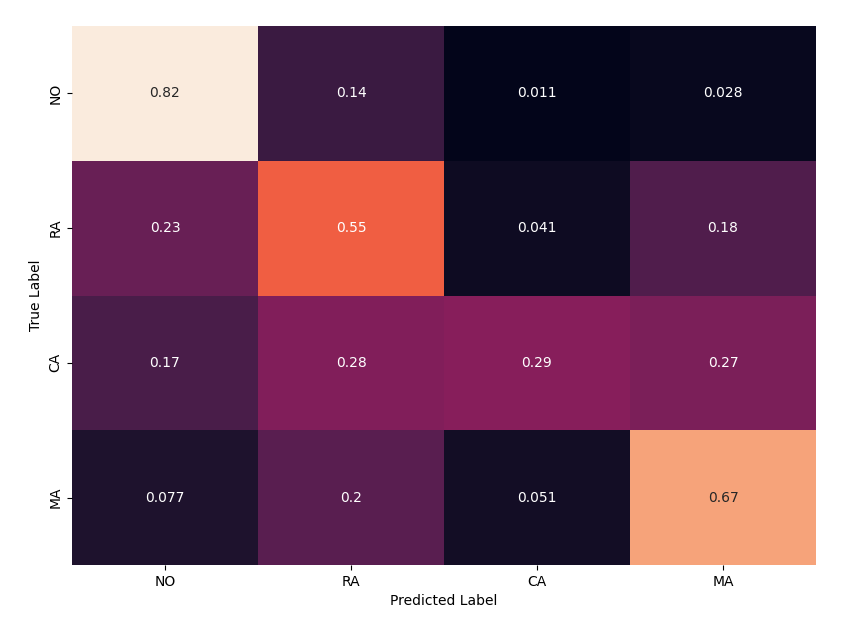
\includegraphics[width=8cm]{text-only-conf-mat-4class}
\caption{Confusion matrix showing true and predicted labels for the text only SCS model.\label{fig:text-only-conf-mat-4class}}
\end{figure}

\subsubsection{The 3-Class Problem}\label{sec:id-3class}

Table \ref{tbl:results-early-3class} shows the macro-f1 scores across
each NO-sampling strategy for the 3-class problem using RoBERTa-base as
the text encoder and Wav2Vec2-base as the audio encoder. Similarly to
the 4-class problem, the addition of acoustic features to not seem to
make an appreciable difference to the performance of the model. However,
it is still useful to discuss the results in more detail, again using
the text only model trained on SCS.

\begin{table}[h]
\centering
\caption{Macro-F1 scores for early sequence fusion models on the 3-class problem. Highest results in each column are shown in bold.\label{tbl:results-early-3class}}
\begin{tabular}{|l|lll|}
\hline
Model         & SCS          & LCS          & US           \\ \hline
Text Only     & \textbf{.62} & .59          & .61          \\
Audio Only    & .21          & .54          & .22          \\ \hline
Concatenation & .61          & .61          & .60          \\
Product       & .58          & .61          & .62          \\
CA Text       & .53          & .53          & .52          \\
CA Audio      & .61          & \textbf{.62} & \textbf{.63} \\ \hline
Random        & .28          & .30          & .29          \\
Majority      & .22          & .22          & .22          \\ \hline
\end{tabular}
\end{table}

Table \ref{tbl:results-seq-3class} shows the results when considering
the different sequence fusion techniques. It can be seen that early
fusion techniques significantly outperform late sequence fusion.
Similarly to the 4-class US run, the early audio only model was not able
to learn during this run. For both the text only and multimodal models,
early fusion improves upon late fusion by approximately 44\%.

\begin{table}[h]
\centering
\caption{Macro-F1 scores across sequence fusion types when trained on SCS on the 3-class problem. \label{tbl:results-seq-3class}}
\begin{tabular}{|l|ll|}
\hline
Model         & Early       & Late      \\ \hline
Text Only     & .62         & .43    \\
Audio Only    & .21         & .33    \\
Concatenation & .61         & .43    \\ \hline
Random        & \multicolumn{2}{c|}{.23} \\
Majority      & \multicolumn{2}{c|}{.15} \\ \hline
\end{tabular}
\end{table}

What follows is a more in-depth analysis of the 3-class in-domain
results. The class F1 distribution for the 3-class problem is shown in
Table \ref{tbl:class-f1-3class}. Similarly to the 4-class F1
distribution, the Attack class appears to be significantly harder to
prodict than the other classes. Similarly to the 4-class problem it can
be hypothesised that this is due to the class imbalance in the dataset.
What is interesting, is the fact that the class F1 scores for the
Attack/CA relations have dropped when compared with the 4-class results
and the scores for non-attack/CA relations have risen. It is possible
that this is simply due to the change in the number of classes, however,
it can also be considered that the 3-class dataset is more heavily
unbalanced against the Attack relation which could also have this
effect.

\begin{table}[h]
\centering
\caption{Class F1 distribution for text only SCS model on test split.\label{tbl:class-f1-3class}}
\begin{tabular}{|lll|}
\hline
None & Support & Attack              \\ \hline
.82         & .78         & .26  \\ \hline
\end{tabular}
\end{table}

The confusion matrix for the 3-class problem, as shown in Figure
\ref{fig:text-only-conf-mat-3class} can also be discussed. Here the
underprediction of the attack class and the overprediction of the
majority class. When compared to the 4-class confusion matrix (Figure
\ref{fig:text-only-conf-mat-4class}) it appears that the model is
effectively combining incorrect predictions between samples labelled
inference and rephrase. This result could imply that the model's
learning is approximately equivalent between the 3- and 4-class
approaches, although it should be noted that more investigation is
required to prove this.

\begin{figure}[h]
\centering
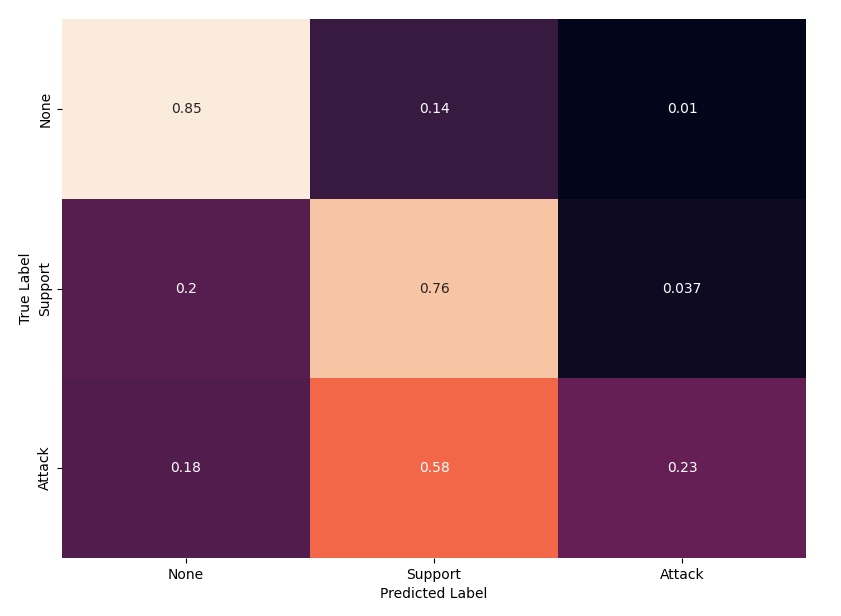
\includegraphics[width=8cm]{text-only-conf-mat-3class}
\caption{Confusion matrix showing true and predicted labels for the text only SCS model.\label{fig:text-only-conf-mat-3class}}
\end{figure}

\subsection{Cross-Domain}\label{sec:res-cd}

In this section the results presented in Section \ref{sec:res-id} are
extended across the Moral Maze subcorpora. Results here are presented
across each subcorpus and the arithmetic mean calculated and also
reported. The goal of this section is to analyse how well the models and
techniques are able to generalise into different topics and domains.
Similar to the In-Domain results, first the 4-class problem is discussed
and then its 3-class equivalent. Only the Macro-F1 scores are reported
here with precision and recall scores added in Appendix
\ref{app:results}.

\subsubsection{The 4-Class Problem}\label{sec:cd-4class}

Table \ref{tbl:cross-4-SCS} provides a cross-domain evaluation of the
different model architectures across the nine Moral Maze subcorpora when
trained on SCS. Taking a broad overview, there is a distinct lack of
significant improvement when the addition of acoustic features is
considered. Since the evaluation is significantly harder than evaluating
in-domain, the models show a significant decrease in the macro-F1 scores
when comparing back to the in-domain results. This drop shows how
challenging it is for the models to generalise effectively across the
different domains.

\begin{table}[h]
\centering
\caption{Mean cross-domain macro-F1 scores for early sequence fusion models on the 4-class problem across different sampling strategies. Highest results in each column are shown in bold.\label{tbl:results-cd-4class-sampling}}
\begin{tabular}{|l|lll|}
\hline
Model         & SCS          & LCS          & US           \\ \hline
Text Only     & .46          & \textbf{.46} & \textbf{.46}          \\
Audio Only    & .37          & .36          & .22          \\ \hline
Concatenation & .45          & .43          & .45          \\
Product       & .45          & .44          & \textbf{.46}          \\
CA Text       & .43          & .32          & .41          \\
CA Audio      & \textbf{.47} & \textbf{.46} & .43 \\ \hline
Random        & .23          & .23          & .23          \\
Majority      & .15          & .15          & .15          \\ \hline
\end{tabular}
\end{table}

\begin{table*}[t]
\centering
\caption{Cross-Domain macro-averaged F1 scores on 4-class SCS trained models. Best scores in each column are shown in bold. \label{tbl:cross-4-SCS}}
\begin{tabular}{|l|llllllll|l|}
\hline
Model         & B            & E            & M            & P            & S            & G            & H            & W            & Mean \\ \hline
Text Only     & .44          & .46          & \textbf{.48} & .42          & .43          & .50          & \textbf{.51} & .41          & .46  \\
Audio Only    & .34          & .37          & .39          & .38          & .33          & .38          & .40          & .37          & .37 \\ \hline
Concatenation & .43          & .43          & .45          & \textbf{.45} & .45          & .49          & .45          & .43          & .45  \\
Product       & .41          & .44          & .42          & .42          & \textbf{.46} & \textbf{.52} & .46          & .43          & .45 \\
CA Text       & .40          & .44          & .44          & .40          & .42          & .49          & .43          & .44          & .43  \\
CA Audio      & \textbf{.45} & \textbf{.49} & .44          & .42          & .45          & .53          & .48          & \textbf{.46} & \textbf{.47}  \\ \hline
Random        & .19          & .23          & .20          & .19          & .22          & .25          & .21          & .24          & .23 \\
Majority      & .16          & .15          & .15          & .15          & .15          & .14          & .15          & .14          & .15  \\ \hline
\end{tabular}
\end{table*}

\begin{table}[h]
\centering
\caption{Macro-F1 scores across sequence fusion types when trained on SCS on the 4-class problem. The mean is taken across all Moral Maze subcorpora. \label{tbl:cross-4-seq}}
\begin{tabular}{|l|ll|}
\hline
Model         & Early       & Late      \\ \hline
Text Only     & .46         & .30       \\
Audio Only    & .37         & .28       \\
Concatenation & .45         & .30       \\ \hline
Random        & \multicolumn{2}{c|}{.23} \\
Majority      & \multicolumn{2}{c|}{.15} \\ \hline
\end{tabular}
\end{table}


\begin{table}[h]
\centering
\caption{Class F1 distribution for text only and CA audio SCS models on banking subcorpus.\label{tbl:class-f1-4class-banking}}
\begin{tabular}{|l|llll|}
\hline
Model     & NO & RA & CA & MA              \\ \hline
Text Only & .67         & .60         & .41         & .065 \\
CA Audio  & .65         & .64         & .41         & .095 \\ \hline
\end{tabular}
\end{table}

Table \ref{tbl:cross-4-seq} compares early and late sequence
fusion in a cross-domain setting. The results reported are the
arithmetic mean across the Moral Maze subcorpora. Generally the increase
is similar to that found in the in-domain evaluation with approximately
a 50\% increase for the text only and multimodal models and a 32\%
increase in performance for the audio only model.

Table \ref{tbl:results-cd-4class-sampling} can be used to compare the
different NO-sampling strategies which again, seem to show little
difference between the various methods, both for unimodal and multimodal
approaches. Similarly to the in-domain results, what follows is a close
look into the results of both the text only and CA audio models when
trained on SCS and evaluated on the Banking subcorpus.

The class F1 distribution can be found in Table
\ref{tbl:class-f1-4class}. Similarly to the in-domain results, the model
is very able to predict unrelated pairs and pairs connected by an
inference, and the score for pairs connected by a conflict are similar.
The major difference in the class distribution is the inability of the
model to accurately predict rephrases, it is possible that this is the
result of an increase in domain specific knowledge and terminology
necessary to predict these rephrases but these data are in no way
conclusive in that respect.

Figures \ref{fig:res-cd-text-banking} and \ref{fig:res-cd-ca-banking}
show the confusion matrices for both the text only model and the CA
audio model when trained on SCS and evaluated on the Banking subcorpus.
While the matrices are generally very similar, there are some notable
differences that show as a trend across all subcorpora. Firstly the
crossmodal attention model is better able to distinguish the rephrases.
The text only model seems to be more likely to predict MA for true CA or
RA samples. The other notable distinction between the two models'
performance is that the text only model is more likely to confuse
conflict-labelled pairs as being unrelated, as opposed to the crossmodal
attention model which is more likely to predict the label as an
inference in all cases. Similarly to the in-domain results, there was no
resampling of the training data that could be found to change the F1
distribution across classes.


\begin{figure}[H]
\centering
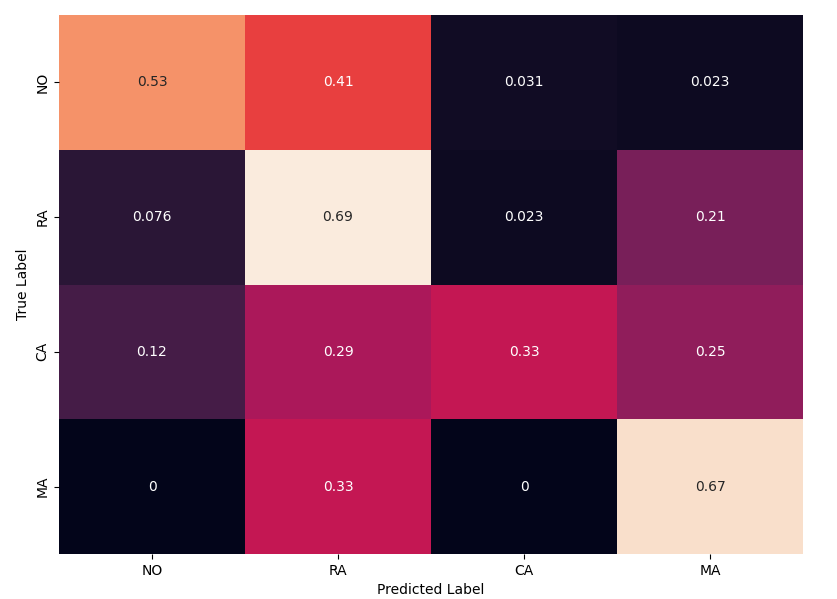
\includegraphics[width=8cm]{ca-audio-conf-mat-4class-banking}
\caption{CA Audio model confusion matrix on the banking subcorpus.\label{fig:res-cd-ca-banking}}
\end{figure}

\begin{figure}[H]
\centering
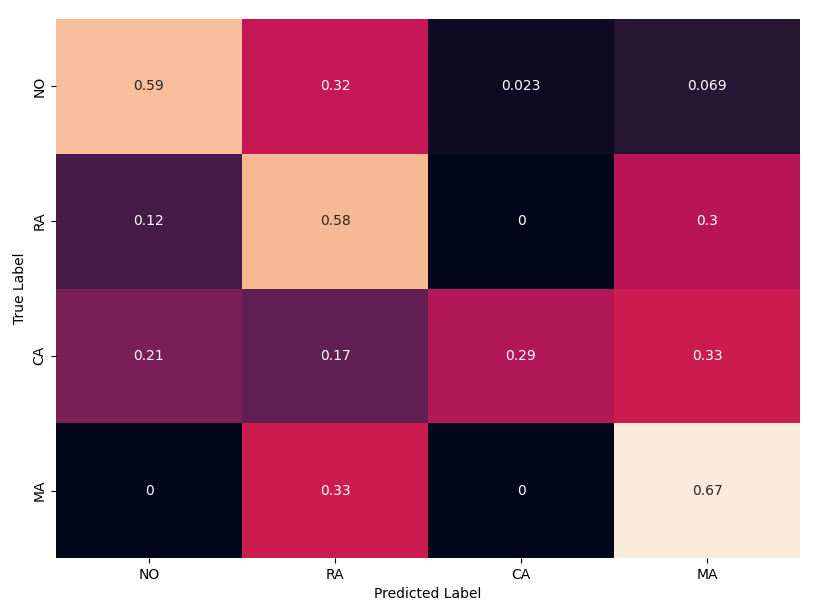
\includegraphics[width=8cm]{text-only-conf-mat-4class-banking}
\caption{Text only model confusion matrix on the banking subcorpus.\label{fig:res-cd-text-banking}}
\end{figure}

\subsubsection{The 3-Class Problem}\label{sec:cd-3class}


Next, the data from the 3-class problem is extended across different
domains. The data can be seen in Table \ref{tbl:cross-3-SCS}. Generally
the results are similar to the 4-class problem with a similar drop in
macro-F1 scores from the in-domain results. Although the 3-class problem
is slightly easier than the 4-class problem, the drop in performance is
still roughly similar.

Table \ref{tbl:results-seq-3class-cd} allows a comparison between early
and late sequence fusion methods on the 3-class problem. Here for both
the text only and multimodal approaches early fusion improves
performance by around 40\% whereas the early audio only model did not
learn effectively. It should be noted that although generally achieving
lower performance, the late fusion models were always able to learn when
only trained on audio data.

\begin{table}[H]
\centering
\caption{Macro-F1 scores across sequence fusion types when trained on SCS on the 3-class problem. The mean is taken across all Moral Maze subcorpora. \label{tbl:results-seq-3class-cd}}
\begin{tabular}{|l|ll|}
\hline
Model         & Early       & Late      \\ \hline
Text Only     & .54         & .38    \\
Audio Only    & .21         & .33    \\
Concatenation & .54         & .40    \\ \hline
Random        & \multicolumn{2}{c|}{.23} \\
Majority      & \multicolumn{2}{c|}{.15} \\ \hline
\end{tabular}
\end{table}

What follows is another discussion regarding the detailed results of the
CA Audio model and the text only model. First, the class F1 distribution
can be found in Table \ref{tbl:class-f1-3class-banking}. Here, as could
reasonably be expected, the results differ significantly from the
4-class problem. The model is able to effectively classify the support
relations and no significant drop is observed when compared to the
in-domain results. However, the drop in macro-F1 seems to originate from
the drop in the model's ability to classify unrelated nodes.

\begin{table}[H]
\centering
\caption{Class F1 distribution for text only and CA audio SCS models on banking subcorpus.\label{tbl:class-f1-3class-banking}}
\begin{tabular}{|l|llll|}
\hline
Model     & None & Support & \multicolumn{1}{l|}{Attack} \\ \hline
Text Only & .66           & .72              & \multicolumn{1}{l|}{.26}         \\
CA Audio  & .58           & .69              & \multicolumn{1}{l|}{.29}         \\ \hline
\end{tabular}
\end{table}

Figure \ref{fig:res-cd-ca-banking-3} shows the confusion matrix for the
CA audio model when evaluated on the banking subcorpus. Much like what
was seen in Section \ref{sec:id-3class} the matrix is characterised by
the overprediction of Support relations, with the main difference being
that this overprediction is worse than when evaluated in-domain.

\begin{figure}[H]
\centering
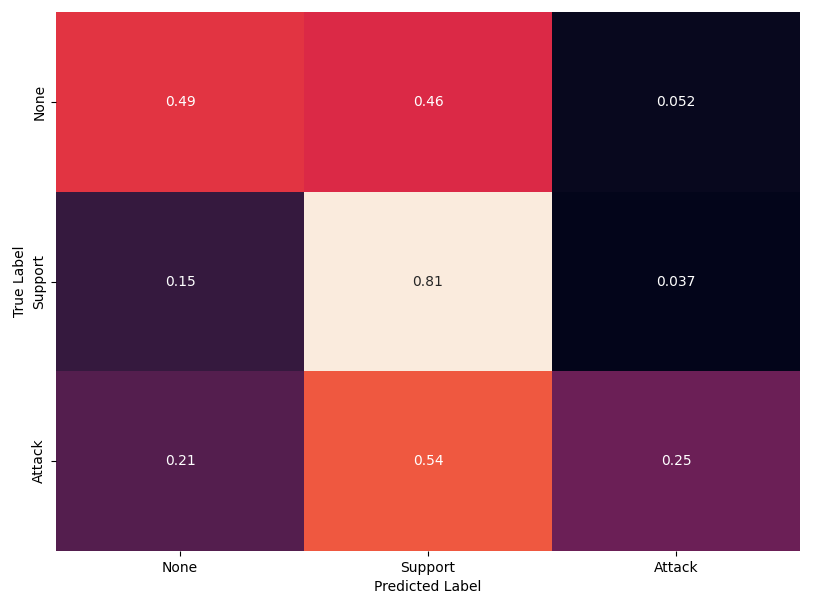
\includegraphics[width=8cm]{ca-audio-conf-mat-3class-banking}
\caption{CA Audio model confusion matrix on the banking subcorpus.\label{fig:res-cd-ca-banking-3}}
\end{figure}

\begin{table*}[t]
\centering
\caption{Cross-Domain macro-averaged F1 scores on 3-class SCS trained models. Best scores in each column are shown in bold. \label{tbl:cross-3-SCS}}
\begin{tabular}{|l|llllllll|l|}
\hline
Model         & B            & E            & M            & P            & S            & G            & H            & W            & Mean  \\ \hline
Text Only     & .54          & .47          & .50          & \textbf{.50} & .58          & .55          & .63          & .51          & \textbf{.54} \\
Audio Only    & .21          & .20          & .22          & .21          & .20          & .21          & .22          & .21          & .21           \\ \hline
Concatenation & .58          & \textbf{.49} & .47          & \textbf{.50} & .57          & \textbf{.57} & .59          & .49          & \textbf{.54} \\
Product       & .51          & .45          & .44          & .47          & .53          & .54          & \textbf{.64} & .47          & .51          \\
CA Text       & .43          & .40          & .43          & .41          & .44          & .46          & .47          & .44          & .44          \\
CA Audio      & \textbf{.59} & .44          & \textbf{.52} & .48          & \textbf{.59} & .54          & .60          & \textbf{.52} & \textbf{.54} \\ \hline
Random        & .27          & .32          & .30          & .27          & .30          & .29          & .29          & .33          & .30          \\
Majority      & .21          & .21          & .22          & .21          & .20          & .21          & .22          & .20          & .21           \\ \hline
\end{tabular}
\end{table*}

\section{Limitations}\label{sec:limitations}

\paragraph{Models}\label{models}

Throughout the project there is a distinct lack of comparison between
different encoder models both from a text and an audio perspective.
While it is likely that the general overarching conclusions would still
hold for other encoders it is very possible that the more specific
conclusions could be encoder-specific. This leads into the fact that
only the base versions of RoBERTa and Wav2Vec2 are used, it has been
shown that using the large models has increased performance both
in-domain and cross-domain for text only tasks {[}15{]}.

\paragraph{Forced Alignment}\label{forced-alignment-1}

Through the use of forced alignment technologies it is very possible for
an amount of accuracy to be lost, especially when considering the poor
environments in which such a system will have to perform in the real
world (i.e.~with lots of crosstalk, a wide range of accents and regional
dialects etc.). While the data presented here have been proven to be
correct to a certain degree, it is not possible to completely guarantee
correctness.

\paragraph{Statistical Significance}\label{statistical-significance}

Because of the time constraints of this project, only a single run could
be performed for each reported result. Therefore it is impossible to
tell whether any comparison is statistically significant, however, given
the size of the major conclusions made it is very likely that they still
hold.

\section{Conclusions}\label{conclusions}

When considering goal (i) as stated in Section \ref{introduction}, as a
result of this project, two major argumentative corpora have been
extended with acoustic features into multimodal datasets for use in many
areas of argumentative research. This includes the large QT30 corpus, of
which a multimodal subset (QT30-MM) is presented, and the much smaller,
cross-domain Moral Maze corpus. QT30-MM is the largest dataset for the ARI task which is currently available.

Goal (ii) of this project was to use the created datasets to conduct an
evaluation of different multimodal techniques in a cross-domain setting,
comparing early and late sequence fusion and various different late
multimodal fusion techniques. Through this evaluation it was found that
the addition of acoustic features does not improve the performance of
argument relation identification systems in-domain and does not improve
the models' ability to generalise across multiple domains.

Although acoustic features were not useful for ARI, it was discovered
that the sequence fusion technique chosen during model creation is
vitally important for the performance of the model. By combining the
sequence data early in the process (before encoding) the model is able
to make cross-sequence dependencies and therefore significantly improves
performance on ARI.

Counterintuitively, all models struggle to distinguish the
attack/conflict relations, it is unclear why this occurs however, since
data augmentation techniques had no effect it appears unlikely that it
is due to the dataset imbalance present. Generally the areas with which
the models struggle do not seem to match human intuition, nor how human
annotators struggle with the task. When considering the cross-domain
results on the 4-class problem, while the models still struggle
distinguishing conflict relations, they struggle even more with
rephrases, often incorrectly predicting conflicts as rephrases, or
predicting rephrases as inferences.

Through the discussion of techniques used to sample unrelated node pairs
they have little difference in-domain indicating that the models are
able to gain the same knowledge and understanding regardless of the
sampling method used, it is simply the difficulty of the evaluation
which changes. This supports previous conclusions that the sampling
method is an important consideration when creating and evaluating ARI
systems {[}51{]}.

The results presented also compare different multimodal fusion
strageties showing that simple concatenation, an elementwise product and
a crossmodal attention mechanism all perform well. The performance of
the crossmodal attention mechanism does vary depending on which modality
is used for queries (and by extension keys and values), it was found
that the mechanism performs best when text is used to generate keys and
values while audio is used to generate the queries.

\section{Future Work}\label{future-work}

To provide a more holistic view of this topic in the future, it would be
useful to further understand the importance of different encoders and
with that whether the varying pre-training strategies have an influence
on the ability of the model to generalise across domains. Another
possible extension would be to consider data processing and
classification methods which preserve inference and conflict structures
as discussed in Section \ref{sec:arg-data}.

With the recent boom in LLMs and especially multimodal LLMs they provide
an opportunity in terms of their potential ability to generalise across
domains with minimal amounts of learning (e.g.~using in-context
learning). LLMs have already shown promise in argument mining tasks so
it seems an appropriate next step to discover how they fair in a
cross-domain environment {[}11{]}.

\section{Legal, Social, Ethical and Professional
Issues}\label{legal-social-ethical-and-professional-issues}

With the recent increases in the availability of AI technologies the
considerations around the ethical, social and professional uses of such systems has
come under scrutiny. Much of this scrutiny relates to how these
intelligent systems can be created and used ethically. Due to the power
of AI systems they are an incredibly useful tool across many fields,
heavily reducing the workload and increasing the productivity of many
people, on the other hand, however, because of this power even
relatively incompetent, malevolent actors have the ability to cause
damage. Before the introduction and increase in the availability of
LLMs, malevalent actors had to be quite competent in order to cause
damage, that has however changed because of the ease of use of such
systems.

It is often possible to cause damage simply through laziness. This has
been seen in the author's previous work in education, where overrelience
on AI systems and assistants can cause a significant decrease in
accuracy, in systems where the use of `human-in-the-loop' type systems
are used with the goal to increase efficiency while still maintaining
accuracy and minimising mistakes. Such a system only works if a. the
tools are used correctly and b. the human does not become complacent and
therefore accuracy falls in relatively critical situations. This is also
a discussion worth having in AM specifically with the release of
interactive assistants for the task {[}61{]}. With the introduction of
openly-useable LLMs such as Open-AI's Chat-GPT models, many people are
using these systems as `life-assistants' and thus this overreliance does
not have bounds in any specific field but rather life as a whole.

Another consideration is the creation and training of such systems,
specifically around the data required. Primarily this comes down to how
the training datasets are sourced, created and annotated (where
annotation is required) and whether this is both legal and ethical. The
details of the annotation of the data used in this project can be found
in the individual datasets' papers, however, it was ensured that all
data from those datasets was annotated and sourced ethically. The
sourcing of data is also an important consideration, especially
surrounding the license under which the original data are released. This
generally becomes a problem when using the data for commercial purposes
(i.e.~creating commercially available models). Throughout this project
it was ensured that all training data has been sourced within the terms
of any licenses.

There is also an environmental implication around training large models,
especially around the power usage when training large models (especially
LLMs). It is therefore important that the power sources are considered
by organisations developing these incredibly large models.

Considering the social implications, LLMs are starting to be used in a
`personal assistant' capacity, including responding to emails or
messages for the user. This immediately produces a lack of trust in the
authenticity of such messages since the goal is generally to talk to the
user.

\section*{Acknowledgements}\label{acknowledgements}
\addcontentsline{toc}{section}{Acknowledgements}

I would like to thank my supervisor Dr.~Ramon Ruiz-Dolz for his
unfailing support and advice throughout this project, and the rest of
the Centre for Argument Technology at the University of Dundee for their
advice and knowledge in the subject. I would also like to thank all of
my friends and family without whom life would be a misery.

\section*{References}\label{references}
\addcontentsline{toc}{section}{References}

\phantomsection\label{refs}
\begin{CSLReferences}{0}{0}
\bibitem[\citeproctext]{ref-lawrenceArgumentMiningSurvey2020}
\CSLLeftMargin{{[}1{]} }%
\CSLRightInline{J. Lawrence and C. Reed, {``Argument {Mining}: {A
Survey},''} \emph{Computational Linguistics}, vol. 45, no. 4, pp.
765--818, Jan. 2020, doi:
\href{https://doi.org/10.1162/coli_a_00364}{10.1162/coli\_a\_00364}.}

\bibitem[\citeproctext]{ref-kotonyaGradualArgumentationEvaluation2019}
\CSLLeftMargin{{[}2{]} }%
\CSLRightInline{N. Kotonya and F. Toni, {``Gradual {Argumentation
Evaluation} for {Stance Aggregation} in {Automated Fake News
Detection},''} in \emph{Proceedings of the 6th {Workshop} on {Argument
Mining}}, Aug. 2019, pp. 156--166. doi:
\href{https://doi.org/10.18653/v1/W19-4518}{10.18653/v1/W19-4518}.}

\bibitem[\citeproctext]{ref-manciniMultimodalFallacyClassification2024}
\CSLLeftMargin{{[}3{]} }%
\CSLRightInline{E. Mancini, F. Ruggeri, and P. Torroni, {``Multimodal
{Fallacy Classification} in {Political Debates},''} in \emph{Proceedings
of the 18th {Conference} of the {European Chapter} of the {Association}
for {Computational Linguistics} ({Volume} 2: {Short Papers})}, Mar.
2024, pp. 170--178.}

\bibitem[\citeproctext]{ref-manciniMultimodalArgumentMining2022}
\CSLLeftMargin{{[}4{]} }%
\CSLRightInline{E. Mancini, F. Ruggeri, A. Galassi, and P. Torroni,
{``Multimodal {Argument Mining}: {A Case Study} in {Political
Debates},''} in \emph{Proceedings of the 9th {Workshop} on {Argument
Mining}}, Oct. 2022, pp. 158--170.}

\bibitem[\citeproctext]{ref-ruiz-dolzVivesDebateSpeechCorpusSpoken2023}
\CSLLeftMargin{{[}5{]} }%
\CSLRightInline{R. Ruiz-Dolz and J. Iranzo-Sánchez,
{``{VivesDebate-Speech}: {A Corpus} of {Spoken Argumentation} to
{Leverage Audio Features} for {Argument Mining},''} in \emph{Proceedings
of the 2023 {Conference} on {Empirical Methods} in {Natural Language
Processing}}, Dec. 2023, pp. 2071--2077. doi:
\href{https://doi.org/10.18653/v1/2023.emnlp-main.128}{10.18653/v1/2023.emnlp-main.128}.}

\bibitem[\citeproctext]{ref-manciniMAMKitComprehensiveMultimodal2024}
\CSLLeftMargin{{[}6{]} }%
\CSLRightInline{E. Mancini, F. Ruggeri, S. Colamonaco, A. Zecca, S.
Marro, and P. Torroni, {``{MAMKit}: {A Comprehensive Multimodal Argument
Mining Toolkit},''} in \emph{Proceedings of the 11th {Workshop} on
{Argument Mining} ({ArgMining} 2024)}, Aug. 2024, pp. 69--82. doi:
\href{https://doi.org/10.18653/v1/2024.argmining-1.7}{10.18653/v1/2024.argmining-1.7}.}

\bibitem[\citeproctext]{ref-mestreMArgMultimodalArgument2021}
\CSLLeftMargin{{[}7{]} }%
\CSLRightInline{R. Mestre, R. Milicin, S. E. Middleton, M. Ryan, J. Zhu,
and T. J. Norman, {``M-{Arg}: {Multimodal Argument Mining Dataset} for
{Political Debates} with {Audio} and {Transcripts},''} in
\emph{Proceedings of the 8th {Workshop} on {Argument Mining}}, Nov.
2021, pp. 78--88. doi:
\href{https://doi.org/10.18653/v1/2021.argmining-1.8}{10.18653/v1/2021.argmining-1.8}.}

\bibitem[\citeproctext]{ref-schneiderWav2vecUnsupervisedPretraining2019}
\CSLLeftMargin{{[}8{]} }%
\CSLRightInline{S. Schneider, A. Baevski, R. Collobert, and M. Auli,
{``Wav2vec: {Unsupervised Pre-training} for {Speech Recognition}.''}
arXiv, Sep. 2019. Accessed: Oct. 17, 2024. {[}Online{]}. Available:
\url{https://arxiv.org/abs/1904.05862}}

\bibitem[\citeproctext]{ref-chenWavLMLargeScaleSelfSupervised2022}
\CSLLeftMargin{{[}9{]} }%
\CSLRightInline{S. Chen \emph{et al.}, {``{WavLM}: {Large-Scale
Self-Supervised Pre-Training} for {Full Stack Speech Processing},''}
\emph{IEEE Journal of Selected Topics in Signal Processing}, vol. 16,
no. 6, pp. 1505--1518, Oct. 2022, doi:
\href{https://doi.org/10.1109/JSTSP.2022.3188113}{10.1109/JSTSP.2022.3188113}.}

\bibitem[\citeproctext]{ref-vaswaniAttentionAllYou2017}
\CSLLeftMargin{{[}10{]} }%
\CSLRightInline{A. Vaswani \emph{et al.}, {``Attention {Is All You
Need},''} p. 11, 2017.}

\bibitem[\citeproctext]{ref-gorurCanLargeLanguage2024}
\CSLLeftMargin{{[}11{]} }%
\CSLRightInline{D. Gorur, A. Rago, and F. Toni, {``Can {Large Language
Models} perform {Relation-based Argument Mining}?''} arXiv, Feb. 2024.
doi:
\href{https://doi.org/10.48550/arXiv.2402.11243}{10.48550/arXiv.2402.11243}.}

\bibitem[\citeproctext]{ref-haddadanYesWeCan2019}
\CSLLeftMargin{{[}12{]} }%
\CSLRightInline{S. Haddadan, E. Cabrio, and S. Villata, {``Yes, we can!
{Mining Arguments} in 50 {Years} of {US Presidential Campaign
Debates},''} in \emph{Proceedings of the 57th {Annual Meeting} of the
{Association} for {Computational Linguistics}}, Jul. 2019, pp.
4684--4690. doi:
\href{https://doi.org/10.18653/v1/P19-1463}{10.18653/v1/P19-1463}.}

\bibitem[\citeproctext]{ref-egerNeuralEndtoEndLearning2017}
\CSLLeftMargin{{[}13{]} }%
\CSLRightInline{S. Eger, J. Daxenberger, and I. Gurevych, {``Neural
{End-to-End Learning} for {Computational Argumentation Mining},''} in
\emph{Proceedings of the 55th {Annual Meeting} of the {Association} for
{Computational Linguistics} ({Volume} 1: {Long Papers})}, Jul. 2017, pp.
11--22. doi:
\href{https://doi.org/10.18653/v1/P17-1002}{10.18653/v1/P17-1002}.}

\bibitem[\citeproctext]{ref-devlinBERTPretrainingDeep2019b}
\CSLLeftMargin{{[}14{]} }%
\CSLRightInline{J. Devlin, M.-W. Chang, K. Lee, and K. Toutanova,
{``{BERT}: {Pre-training} of {Deep Bidirectional Transformers} for
{Language Understanding}.''} arXiv, May 2019. doi:
\href{https://doi.org/10.48550/arXiv.1810.04805}{10.48550/arXiv.1810.04805}.}

\bibitem[\citeproctext]{ref-ruiz-dolzTransformerBasedModelsAutomatic2021}
\CSLLeftMargin{{[}15{]} }%
\CSLRightInline{R. Ruiz-Dolz, J. Alemany, S. M. H. Barberá, and A.
García-Fornes, {``Transformer-{Based Models} for {Automatic
Identification} of {Argument Relations}: {A Cross-Domain Evaluation},''}
\emph{IEEE Intelligent Systems}, vol. 36, no. 6, pp. 62--70, Nov. 2021,
doi:
\href{https://doi.org/10.1109/MIS.2021.3073993}{10.1109/MIS.2021.3073993}.}

\bibitem[\citeproctext]{ref-gemechuARIESGeneralBenchmark2024}
\CSLLeftMargin{{[}16{]} }%
\CSLRightInline{D. Gemechu, R. Ruiz-Dolz, and C. Reed, {``{ARIES}: {A
General Benchmark} for {Argument Relation Identification},''} in
\emph{Proceedings of the 11th {Workshop} on {Argument Mining}
({ArgMining} 2024)}, Aug. 2024, pp. 1--14. doi:
\href{https://doi.org/10.18653/v1/2024.argmining-1.1}{10.18653/v1/2024.argmining-1.1}.}

\bibitem[\citeproctext]{ref-hautli-janiszQT30CorpusArgument2022}
\CSLLeftMargin{{[}17{]} }%
\CSLRightInline{A. Hautli-Janisz, Z. Kikteva, W. Siskou, K. Gorska, R.
Becker, and C. Reed, {``{QT30}: {A Corpus} of {Argument} and {Conflict}
in {Broadcast Debate},''} in \emph{Proceedings of the {Thirteenth
Language Resources} and {Evaluation Conference}}, Jun. 2022, pp.
3291--3300.}

\bibitem[\citeproctext]{ref-lawrenceAIFdbCorpora2014}
\CSLLeftMargin{{[}18{]} }%
\CSLRightInline{J. Lawrence and C. Reed, {``{AIFdb Corpora},''} in
\emph{Frontiers in {Artificial Intelligence} and {Applications}}, IOS
Press, 2014. doi:
\href{https://doi.org/10.3233/978-1-61499-436-7-465}{10.3233/978-1-61499-436-7-465}.}

\bibitem[\citeproctext]{ref-hamblinFallacies1970}
\CSLLeftMargin{{[}19{]} }%
\CSLRightInline{C. L. Hamblin, \emph{Fallacies}, First Edition. London:
Methuen young books, 1970.}

\bibitem[\citeproctext]{ref-searleSpeechActsEssay1969}
\CSLLeftMargin{{[}20{]} }%
\CSLRightInline{J. R. Searle, \emph{Speech {Acts}: {An Essay} in the
{Philosophy} of {Language}}. Cambridge: Cambridge University Press,
1969. doi:
\href{https://doi.org/10.1017/CBO9781139173438}{10.1017/CBO9781139173438}.}

\bibitem[\citeproctext]{ref-mannRhetoricalStructureTheory1988}
\CSLLeftMargin{{[}21{]} }%
\CSLRightInline{W. C. Mann and S. A. Thompson, {``Rhetorical {Structure
Theory}: {Toward} a functional theory of text organization,''}
\emph{Text - Interdisciplinary Journal for the Study of Discourse}, vol.
8, no. 3, pp. 243--281, Jan. 1988, doi:
\href{https://doi.org/10.1515/text.1.1988.8.3.243}{10.1515/text.1.1988.8.3.243}.}

\bibitem[\citeproctext]{ref-reedHowDialoguesCreate2011}
\CSLLeftMargin{{[}22{]} }%
\CSLRightInline{C. Reed and K. Budzynska, {``How dialogues create
arguments,''} 2011.}

\bibitem[\citeproctext]{ref-reedQuickStartGuide2017}
\CSLLeftMargin{{[}23{]} }%
\CSLRightInline{C. Reed, {``A {Quick Start Guide} to {Inference
Anchoring Theory} ({IAT}).''} Sep. 2017.}

\bibitem[\citeproctext]{ref-waltonArgumentationSchemes2008}
\CSLLeftMargin{{[}24{]} }%
\CSLRightInline{D. Walton, C. Reed, and F. Macagno, \emph{Argumentation
{Schemes}}. Cambridge: Cambridge University Press, 2008. doi:
\href{https://doi.org/10.1017/CBO9780511802034}{10.1017/CBO9780511802034}.}

\bibitem[\citeproctext]{ref-waltonArgumentationTheoryVery2009}
\CSLLeftMargin{{[}25{]} }%
\CSLRightInline{D. Walton, {``Argumentation {Theory}: {A Very Short
Introduction},''} in \emph{Argumentation in {Artificial Intelligence}},
G. Simari and I. Rahwan, Eds. Boston, MA: Springer US, 2009, pp. 1--22.
doi:
\href{https://doi.org/10.1007/978-0-387-98197-0_1}{10.1007/978-0-387-98197-0\_1}.}

\bibitem[\citeproctext]{ref-budzynskaModelProcessingIllocutionary2014}
\CSLLeftMargin{{[}26{]} }%
\CSLRightInline{K. Budzynska, M. Janier, C. Reed, P. Saint-Dizier, M.
Stede, and O. Yakorska, {``A {Model} for {Processing Illocutionary
Structures} and {Argumentation} in {Debates},''} in \emph{Proceedings of
the {Ninth International Conference} on {Language Resources} and
{Evaluation} ({LREC}`14)}, May 2014, pp. 917--924.}

\bibitem[\citeproctext]{ref-reedAraucariaSoftwareArgument2004}
\CSLLeftMargin{{[}27{]} }%
\CSLRightInline{C. Reed and G. Rowe, {``Araucaria: Software for argument
analysis, diagramming and representation,''} \emph{International Journal
on Artificial Intelligence Tools}, vol. 13, no. 4, pp. 961--979, Dec.
2004, doi:
\href{https://doi.org/10.1142/S0218213004001922}{10.1142/S0218213004001922}.}

\bibitem[\citeproctext]{ref-chesnevarArgumentInterchangeFormat2006}
\CSLLeftMargin{{[}28{]} }%
\CSLRightInline{C. Chesñevar \emph{et al.}, {``Towards an argument
interchange format,''} \emph{The Knowledge Engineering Review}, vol. 21,
no. 4, pp. 293--316, Dec. 2006, doi:
\href{https://doi.org/10.1017/S0269888906001044}{10.1017/S0269888906001044}.}

\bibitem[\citeproctext]{ref-reedAIFDialogueArgument}
\CSLLeftMargin{{[}29{]} }%
\CSLRightInline{C. Reed, J. Devereux, S. Wells, and G. Rowe, {``{AIF}+:
{Dialogue} in the {Argument Interchange Format}.''}}

\bibitem[\citeproctext]{ref-rahwanLayingFoundationsWorld2007}
\CSLLeftMargin{{[}30{]} }%
\CSLRightInline{I. Rahwan, F. Zablith, and C. Reed, {``Laying the
foundations for a {World Wide Argument Web},''} \emph{Artificial
Intelligence}, vol. 171, no. 10--15, pp. 897--921, Jul. 2007, doi:
\href{https://doi.org/10.1016/j.artint.2007.04.015}{10.1016/j.artint.2007.04.015}.}

\bibitem[\citeproctext]{ref-lawrenceAIFdbInfrastructureArgument2012}
\CSLLeftMargin{{[}31{]} }%
\CSLRightInline{J. Lawrence, F. Bex, C. Reed, and M. Snaith, {``{AIFdb}:
{Infrastructure} for the {Argument Web},''} in \emph{Computational
{Models} of {Argument}}, IOS Press, 2012, pp. 515--516. doi:
\href{https://doi.org/10.3233/978-1-61499-111-3-515}{10.3233/978-1-61499-111-3-515}.}

\bibitem[\citeproctext]{ref-petersDeepContextualizedWord2018}
\CSLLeftMargin{{[}32{]} }%
\CSLRightInline{M. E. Peters \emph{et al.}, {``Deep contextualized word
representations.''} arXiv, Mar. 2018. doi:
\href{https://doi.org/10.48550/arXiv.1802.05365}{10.48550/arXiv.1802.05365}.}

\bibitem[\citeproctext]{ref-daiSemisupervisedSequenceLearning2015}
\CSLLeftMargin{{[}33{]} }%
\CSLRightInline{A. M. Dai and Q. V. Le, {``Semi-supervised {Sequence
Learning}.''} arXiv, Nov. 2015. doi:
\href{https://doi.org/10.48550/arXiv.1511.01432}{10.48550/arXiv.1511.01432}.}

\bibitem[\citeproctext]{ref-liuRoBERTaRobustlyOptimized2019a}
\CSLLeftMargin{{[}34{]} }%
\CSLRightInline{Y. Liu \emph{et al.}, {``{RoBERTa}: {A Robustly
Optimized BERT Pretraining Approach}.''} arXiv, Jul. 2019. doi:
\href{https://doi.org/10.48550/arXiv.1907.11692}{10.48550/arXiv.1907.11692}.}

\bibitem[\citeproctext]{ref-openaiGPT4TechnicalReport2024}
\CSLLeftMargin{{[}35{]} }%
\CSLRightInline{OpenAI \emph{et al.}, {``{GPT-4 Technical Report}.''}
arXiv, Mar. 2024. doi:
\href{https://doi.org/10.48550/arXiv.2303.08774}{10.48550/arXiv.2303.08774}.}

\bibitem[\citeproctext]{ref-touvronLLaMAOpenEfficient2023}
\CSLLeftMargin{{[}36{]} }%
\CSLRightInline{H. Touvron \emph{et al.}, {``{LLaMA}: {Open} and
{Efficient Foundation Language Models}.''} arXiv, Feb. 2023. doi:
\href{https://doi.org/10.48550/arXiv.2302.13971}{10.48550/arXiv.2302.13971}.}

\bibitem[\citeproctext]{ref-brownLanguageModelsAre2020}
\CSLLeftMargin{{[}37{]} }%
\CSLRightInline{T. B. Brown \emph{et al.}, {``Language {Models} are
{Few-Shot Learners}.''} arXiv, Jul. 2020. doi:
\href{https://doi.org/10.48550/arXiv.2005.14165}{10.48550/arXiv.2005.14165}.}

\bibitem[\citeproctext]{ref-sharmaArgumentativeStancePrediction2023}
\CSLLeftMargin{{[}38{]} }%
\CSLRightInline{A. Sharma, A. Gupta, and M. Bilalpur, {``Argumentative
{Stance Prediction}: {An Exploratory Study} on {Multimodality} and
{Few-Shot Learning},''} in \emph{Proceedings of the 10th {Workshop} on
{Argument Mining}}, Dec. 2023, pp. 167--174. doi:
\href{https://doi.org/10.18653/v1/2023.argmining-1.18}{10.18653/v1/2023.argmining-1.18}.}

\bibitem[\citeproctext]{ref-baevskiWav2vec20Framework2020}
\CSLLeftMargin{{[}39{]} }%
\CSLRightInline{A. Baevski, H. Zhou, A. Mohamed, and M. Auli, {``Wav2vec
2.0: {A Framework} for {Self-Supervised Learning} of {Speech
Representations}.''} arXiv, Oct. 2020. Accessed: Oct. 16, 2024.
{[}Online{]}. Available: \url{https://arxiv.org/abs/2006.11477}}

\bibitem[\citeproctext]{ref-hsuHuBERTSelfSupervisedSpeech2021}
\CSLLeftMargin{{[}40{]} }%
\CSLRightInline{W.-N. Hsu, B. Bolte, Y.-H. H. Tsai, K. Lakhotia, R.
Salakhutdinov, and A. Mohamed, {``{HuBERT}: {Self-Supervised Speech
Representation Learning} by {Masked Prediction} of {Hidden Units}.''}
arXiv, Jun. 2021. doi:
\href{https://doi.org/10.48550/arXiv.2106.07447}{10.48550/arXiv.2106.07447}.}

\bibitem[\citeproctext]{ref-delbrouckViLMedicFrameworkResearch2022}
\CSLLeftMargin{{[}41{]} }%
\CSLRightInline{J. Delbrouck \emph{et al.}, {``{ViLMedic}: A framework
for research at the intersection of vision and language in medical
{AI},''} in \emph{Proceedings of the 60th {Annual Meeting} of the
{Association} for {Computational Linguistics}: {System Demonstrations}},
May 2022, pp. 23--34. doi:
\href{https://doi.org/10.18653/v1/2022.acl-demo.3}{10.18653/v1/2022.acl-demo.3}.}

\bibitem[\citeproctext]{ref-sunCMAFNetCrossmodalAttention2024}
\CSLLeftMargin{{[}42{]} }%
\CSLRightInline{K. Sun \emph{et al.}, {``{CMAF-Net}: A cross-modal
attention fusion-based deep neural network for incomplete multi-modal
brain tumor segmentation,''} \emph{Quantitative Imaging in Medicine and
Surgery}, vol. 14, no. 7, pp. 4579--4604, Jul. 2024, doi:
\href{https://doi.org/10.21037/qims-24-9}{10.21037/qims-24-9}.}

\bibitem[\citeproctext]{ref-totoAudiBERTDeepTransfer2021}
\CSLLeftMargin{{[}43{]} }%
\CSLRightInline{E. Toto, M. Tlachac, and E. A. Rundensteiner,
{``{AudiBERT}: {A Deep Transfer Learning Multimodal Classification
Framework} for {Depression Screening},''} in \emph{Proceedings of the
30th {ACM International Conference} on {Information} \& {Knowledge
Management}}, Oct. 2021, pp. 4145--4154. doi:
\href{https://doi.org/10.1145/3459637.3481895}{10.1145/3459637.3481895}.}

\bibitem[\citeproctext]{ref-tsaiMultimodalTransformerUnaligned2019}
\CSLLeftMargin{{[}44{]} }%
\CSLRightInline{Y.-H. H. Tsai, S. Bai, P. P. Liang, J. Z. Kolter, L.-P.
Morency, and R. Salakhutdinov, {``Multimodal {Transformer} for
{Unaligned Multimodal Language Sequences},''} in \emph{Proceedings of
the 57th {Annual Meeting} of the {Association} for {Computational
Linguistics}}, Jul. 2019, pp. 6558--6569. doi:
\href{https://doi.org/10.18653/v1/P19-1656}{10.18653/v1/P19-1656}.}

\bibitem[\citeproctext]{ref-rajanCrossAttentionPreferableSelfAttention2022}
\CSLLeftMargin{{[}45{]} }%
\CSLRightInline{V. Rajan, A. Brutti, and A. Cavallaro, {``Is
{Cross-Attention Preferable} to {Self-Attention} for {Multi-Modal
Emotion Recognition}?''} arXiv, Feb. 2022. doi:
\href{https://doi.org/10.48550/arXiv.2202.09263}{10.48550/arXiv.2202.09263}.}

\bibitem[\citeproctext]{ref-yeCrossModalSelfAttentionNetwork2019}
\CSLLeftMargin{{[}46{]} }%
\CSLRightInline{L. Ye, M. Rochan, Z. Liu, and Y. Wang, {``Cross-{Modal
Self-Attention Network} for {Referring Image Segmentation}.''} arXiv,
Apr. 2019. doi:
\href{https://doi.org/10.48550/arXiv.1904.04745}{10.48550/arXiv.1904.04745}.}

\bibitem[\citeproctext]{ref-wuKnowCompDialAM2024Finetuning2024}
\CSLLeftMargin{{[}47{]} }%
\CSLRightInline{Y. Wu, Y. Zhou, B. Xu, W. Wang, and Y. Song,
{``{KnowComp} at {DialAM-2024}: {Fine-tuning Pre-trained Language
Models} for {Dialogical Argument Mining} with {Inference Anchoring
Theory},''} in \emph{Proceedings of the 11th {Workshop} on {Argument
Mining} ({ArgMining} 2024)}, Aug. 2024, pp. 103--109. doi:
\href{https://doi.org/10.18653/v1/2024.argmining-1.10}{10.18653/v1/2024.argmining-1.10}.}

\bibitem[\citeproctext]{ref-zhengKNOWCOMPPOKEMONTeam2024}
\CSLLeftMargin{{[}48{]} }%
\CSLRightInline{Z. Zheng, Z. Wang, Q. Zong, and Y. Song, {``{KNOWCOMP
POKEMON Team} at {DialAM-2024}: {A Two-Stage Pipeline} for {Detecting
Relations} in {Dialogue Argument Mining},''} in \emph{Proceedings of the
11th {Workshop} on {Argument Mining} ({ArgMining} 2024)}, Aug. 2024, pp.
110--118. doi:
\href{https://doi.org/10.18653/v1/2024.argmining-1.11}{10.18653/v1/2024.argmining-1.11}.}

\bibitem[\citeproctext]{ref-stabCrosstopicArgumentMining2018}
\CSLLeftMargin{{[}49{]} }%
\CSLRightInline{C. Stab, T. Miller, B. Schiller, P. Rai, and I.
Gurevych, {``Cross-topic {Argument Mining} from {Heterogeneous
Sources},''} in \emph{Proceedings of the 2018 {Conference} on {Empirical
Methods} in {Natural Language Processing}}, Oct. 2018, pp. 3664--3674.
doi: \href{https://doi.org/10.18653/v1/D18-1402}{10.18653/v1/D18-1402}.}

\bibitem[\citeproctext]{ref-al-khatibCrossDomainMiningArgumentative2016}
\CSLLeftMargin{{[}50{]} }%
\CSLRightInline{K. Al-Khatib, H. Wachsmuth, M. Hagen, J. Köhler, and B.
Stein, {``Cross-{Domain Mining} of {Argumentative Text} through {Distant
Supervision},''} in \emph{Proceedings of the 2016 {Conference} of the
{North American Chapter} of the {Association} for {Computational
Linguistics}: {Human Language Technologies}}, Jun. 2016, pp. 1395--1404.
doi: \href{https://doi.org/10.18653/v1/N16-1165}{10.18653/v1/N16-1165}.}

\bibitem[\citeproctext]{ref-ruiz-dolzLookingUnseenEffective2025}
\CSLLeftMargin{{[}51{]} }%
\CSLRightInline{R. Ruiz-Dolz, D. Gemechu, Z. Kikteva, and C. Reed,
{``Looking at the {Unseen}: {Effective Sampling} of {Non-Related
Propositions} for {Argument Mining},''} in \emph{Proceedings of the 31st
{International Conference} on {Computational Linguistics}}, Jan. 2025,
pp. 2131--2143.}

\bibitem[\citeproctext]{ref-liuImageArgMultimodalTweet2022}
\CSLLeftMargin{{[}52{]} }%
\CSLRightInline{Z. Liu, M. Guo, Y. Dai, and D. Litman, {``{ImageArg}: {A
Multi-modal Tweet Dataset} for {Image Persuasiveness Mining},''} in
\emph{Proceedings of the 9th {Workshop} on {Argument Mining}}, Oct.
2022, pp. 1--18.}

\bibitem[\citeproctext]{ref-zongTILFAUnifiedFramework2023}
\CSLLeftMargin{{[}53{]} }%
\CSLRightInline{Q. Zong \emph{et al.}, {``{TILFA}: {A Unified Framework}
for {Text}, {Image}, and {Layout Fusion} in {Argument Mining},''} in
\emph{Proceedings of the 10th {Workshop} on {Argument Mining}}, Dec.
2023, pp. 139--147. doi:
\href{https://doi.org/10.18653/v1/2023.argmining-1.14}{10.18653/v1/2023.argmining-1.14}.}

\bibitem[\citeproctext]{ref-liuOverviewImageArg2023First2023}
\CSLLeftMargin{{[}54{]} }%
\CSLRightInline{Z. Liu, M. Elaraby, Y. Zhong, and D. Litman, {``Overview
of {ImageArg-2023}: {The First Shared Task} in {Multimodal Argument
Mining},''} in \emph{Proceedings of the 10th {Workshop} on {Argument
Mining}}, Dec. 2023, pp. 120--132. doi:
\href{https://doi.org/10.18653/v1/2023.argmining-1.12}{10.18653/v1/2023.argmining-1.12}.}

\bibitem[\citeproctext]{ref-gravesConnectionistTemporalClassification2006}
\CSLLeftMargin{{[}55{]} }%
\CSLRightInline{A. Graves, S. Fernández, F. Gomez, and J. Schmidhuber,
{``Connectionist temporal classification: Labelling unsegmented sequence
data with recurrent neural networks,''} in \emph{Proceedings of the 23rd
international conference on {Machine} learning - {ICML} '06}, 2006, pp.
369--376. doi:
\href{https://doi.org/10.1145/1143844.1143891}{10.1145/1143844.1143891}.}

\bibitem[\citeproctext]{ref-lippiArgumentMiningSpeech2016}
\CSLLeftMargin{{[}56{]} }%
\CSLRightInline{M. Lippi and P. Torroni, {``Argument {Mining} from
{Speech}: {Detecting Claims} in {Political Debates},''}
\emph{Proceedings of the AAAI Conference on Artificial Intelligence},
vol. 30, no. 1, Mar. 2016, doi:
\href{https://doi.org/10.1609/aaai.v30i1.10384}{10.1609/aaai.v30i1.10384}.}

\bibitem[\citeproctext]{ref-manciniMultimodalFallacyClassification2024a}
\CSLLeftMargin{{[}57{]} }%
\CSLRightInline{E. Mancini, F. Ruggeri, and P. Torroni, {``Multimodal
{Fallacy Classification} in {Political Debates},''} in \emph{Proceedings
of the 18th {Conference} of the {European Chapter} of the {Association}
for {Computational Linguistics} ({Volume} 2: {Short Papers})}, Mar.
2024, pp. 170--178.}

\bibitem[\citeproctext]{ref-loshchilovDecoupledWeightDecay2019a}
\CSLLeftMargin{{[}58{]} }%
\CSLRightInline{I. Loshchilov and F. Hutter, {``Decoupled {Weight Decay
Regularization}.''} arXiv, Jan. 2019. doi:
\href{https://doi.org/10.48550/arXiv.1711.05101}{10.48550/arXiv.1711.05101}.}

\bibitem[\citeproctext]{ref-junsomboonCombiningOverSamplingUnderSampling2017}
\CSLLeftMargin{{[}59{]} }%
\CSLRightInline{N. Junsomboon and T. Phienthrakul, {``Combining
{Over-Sampling} and {Under-Sampling Techniques} for {Imbalance
Dataset},''} in \emph{Proceedings of the 9th {International Conference}
on {Machine Learning} and {Computing}}, Feb. 2017, pp. 243--247. doi:
\href{https://doi.org/10.1145/3055635.3056643}{10.1145/3055635.3056643}.}

\bibitem[\citeproctext]{ref-mohammedMachineLearningOversampling2020}
\CSLLeftMargin{{[}60{]} }%
\CSLRightInline{R. Mohammed, J. Rawashdeh, and M. Abdullah, {``Machine
{Learning} with {Oversampling} and {Undersampling Techniques}: {Overview
Study} and {Experimental Results},''} in \emph{2020 11th {International
Conference} on {Information} and {Communication Systems} ({ICICS})},
Apr. 2020, pp. 243--248. doi:
\href{https://doi.org/10.1109/ICICS49469.2020.239556}{10.1109/ICICS49469.2020.239556}.}

\bibitem[\citeproctext]{ref-lenzArgueMapperAssistantInteractive2025}
\CSLLeftMargin{{[}61{]} }%
\CSLRightInline{M. Lenz and R. Bergmann, {``{ArgueMapper Assistant}:
{Interactive Argument Mining Using Generative Language Models},''} in
\emph{Artificial {Intelligence XLI}}, 2025, pp. 189--203. doi:
\href{https://doi.org/10.1007/978-3-031-77915-2_14}{10.1007/978-3-031-77915-2\_14}.}

\end{CSLReferences}

\appendix

\section{Datasets}\label{app:datasets}

\section{Results}\label{app:results}

\section{Ethics Declaration}\label{ethics-declaration}

\section{Risk Assessment}\label{risk-assessment}

\section{Mid-Term Report}\label{mid-term-report}

\section{Poster and Demonstration
Materials}\label{poster-and-demonstration-materials}

%%%%%%%%%%%
%%%%%%%%%%%


% END DOCUMENT
\end{document}
